\section{Data Driven QCD Determination}
\label{sec:dataDrivenQCD}
% ---- ---- ---- ---- ---- ---- ---- ---- ---- ---- ---- ---- ---- ---- ---- ---- ---- ---- ---- ---- ---- ---- ----

A background from QCD multijet events comes from 3- or 4-jet events
with one jet passing the lepton criteria as a 'fake'. However, it is
not practical to generate sufficient MC to create a statistically
significant sample that passes the selection criteria. Therefore, we
rely on a data-driven approach in which the isolation-inverted samples
from data, which mirror the QCD background, are used instead.
Specifically, we perform a two-component simultaneous fit to data of
the MET distribution in order to obtain the fraction of QCD events in
the data; the two components are a data-based QCD sample and a
MC-based W+Jets sample.

The electron QCD sample is obtained by selecting events
in the data with the isolation $>0.3$ (default selection for loose
electrons uses Iso$_{el}<\sim0.2$).  In order to increase statistics
for the QCD sample we also relax the MET cut from 30~GeV to 20~GeV and
remove the restrictions on Electron MVA.
Fig.~\ref{fig:QCDISOCutsWmTShape} demonstrates that taking $Iso>0.3$
(rather than simply inverting the isolation cut), relaxing the MET as
well as the Electron MVA gives us a falling $W_{mT}$ spectrum (as
opposed to a signal-like one, which contains a peak near
$W_{mT}=80$GeV). The MC W+Jets and target data samples are obtained by
applying the default cuts (Sec~\ref{sec:firstStep}).

The fraction of QCD events in data is then obtained from a
fit to the MET distribution, with the normalizations for two components (
W+jets and QCD) free to float.
The results for the electrons are shown in Figure~\ref{fig:QCDTemplateFit_MET}. 
However, we inherently have a smaller sample of 
QCD events for the muons. Their relative fraction
is taken from the fit to the 7TeV data (AN-11-110).
Due to this assumption, to account for discrepancies in template modeling
(e.g. using W+jets MC as a proxy for all non-QCD processes) as well as the
fact that the QCD fraction is estimated prior to the MVA cut, a very
large uncertainty is conservatively assumed. The final fraction of QCD
events in data, after accounting for the change in accepatance due to the MET cut,
are given in Table~\ref{tab:qcdfrac}. They are fed to the $m_{jj}$ fit for determination of the QCD
normalization, and the four-body shape of the QCD distribution is fed
to the final four-body total background determination in preparation
for the limit setting procedure.

%%Note that the W transverse mass distributions from the data and MC are
%%statistically consistent, as shown in
%%Figure~\ref{fig:QCDCutLoosening_MET} for muons; for electrons there's
%%an insufficient number of MC events to make the comparison.  The MET
%%for QCD processes is also 'fake'; i.e., it originates from badly
%%measured jets, and therefore has an exponentially falling spectrum.
%%By contrast, all other backgrounds exhibit a wide peak at $\sim
%%35$~GeV from a real neutrino (with the exception of Z+Jets, where the
%%MET is the result of a poorly measured lepton).

%%  $el_{2J}$ $frac_{QCD}=0.0617\pm 0.00384$,
%%  $el_{3J}$ $frac_{QCD}=0.0213\pm 0.00678$.
%%
%% $\mu_{2J}$ $frac_{QCD}=0.001625\pm 0.004214$,
%% $\mu_{3J}$ $frac_{QCD}=0.0\pm 0.0040797$,


\begin{table}[bthp]
\begin{center}
  \begin{tabular}{l c}
    \hline  \hline
     & 2 jets \\
    \hline  
    electron  & 17.0 $\pm$ 0.2\% \\
    muon      & 0.2 $\pm$ 0.4\% \\
    \hline  \hline
  \end{tabular}
\end{center}
\caption{\label{tab:qcdfrac} Estimates of the percentage of QCD in data (and
the fit uncertainty) for the muon and electron datasets after selection.}
\end{table}

\subsection{QCD Uncertainties}
\label{sec:qcd_Uncertainty}
% .... .... .... .... .... .... .... .... .... .... .... .... .... .... .... .... .... .... .... .... .... .... ....

When performing the $m_{jj}$ fit the QCD yield
is Gaussian-constrained with a mean given by the value shown in
Table~\ref{tab:qcdfrac}.
In the case of electrons, the error on the QCD fraction
is small and we (conservatively) estimate
the uncertainty to be one half of the expected value. For muons the
uncertainty is the error on the relative fraction (i.e.,
0.4\%).
When fitting the sum of electron and muon data, the uncertainties
are combined using the standard error propagation machinery.


\subsection{Cross-Checks}

In order to ensure that our inverted selection provides a consistent representation of
QCD events,
we fit the QCD with a Raileigh Function: $xe^{-x^2/2(\sigma_0+\sigma_1x)^2}$,
used during the inclusive cross section measurements~\cite{WZCMS:2010}.
As can be seen from Fig.~\ref{fig:QCDMETRaileighFit},
the function accurately fits the overall shape as well as the parameter
corresponding to the intrinsic MET resolution ($\sigma_0\simeq 12$~GeV).

In addition we compare the above procedure to the fit with the remaining backgrounds included by
\begin{itemize}
\item Fixing the relative ratios based on the expected cross sections and fitting with the combination, instead of W+Jets. The resulting fraction of QCD (after correcting for MET acceptance) is $0.145\pm 0.002$.
\item Fixing the additional backgrounds to their expected values and only allowing W+Jets (and QCD) to float during the fit. The resulting fraction of QCD (after correcting for MET acceptance) is $0.139\pm 0.002$.
\end{itemize}
The results (Fig.~\ref{fig:QCDTemplateFit_MET_AllBkgds}) are consistent with the default approach.


% we perform the following cross-checks:
% \begin{itemize}
% \item Fit the QCD with a Raileigh Function: $xe^{-x^2/2(\sigma_0+\sigma_1x)^2}$,
% used during the inclusive cross section measurements~\cite{WZCMS:2010}.
% As can be seen from Fig.~\ref{fig:QCDMETRaileighFit},
% the function accurately fits the overall shape as well as the parameter
% corresponding to the intrinsic MET resolution ($\sigma_0\simeq 10$~GeV).
% \item Compare the W transverse mass shapes for the data sidebands with MET$>20$~GeV vs
% MET$>30$~GeV (Fig.~\ref{fig:QCDMETCutsWmTShape}). Naturally, events with MET$>30$~GeV do not have the
% same exponential falloff, since they contain a higher percentage of W's.
% \item Examine the impact of setting Iso$>0.1$, rather than Iso$>0.2$.
% We compare the MET (Fig.~\ref{fig:QCDISOCutsMETShape}) and W transverse mass
% (Fig.~\ref{fig:QCDISOCutsWmTShape}) distributions, and conclude that there is no statistically
% significant discrepancy introduced by the looser isolation requirement.
% \end{itemize}


%%%%%%%%%%%%%%%%%%%%%%%%%%%%
%%%%%%%
%\begin{figure}[h!] {\centering
%\unitlength=0.33\linewidth
%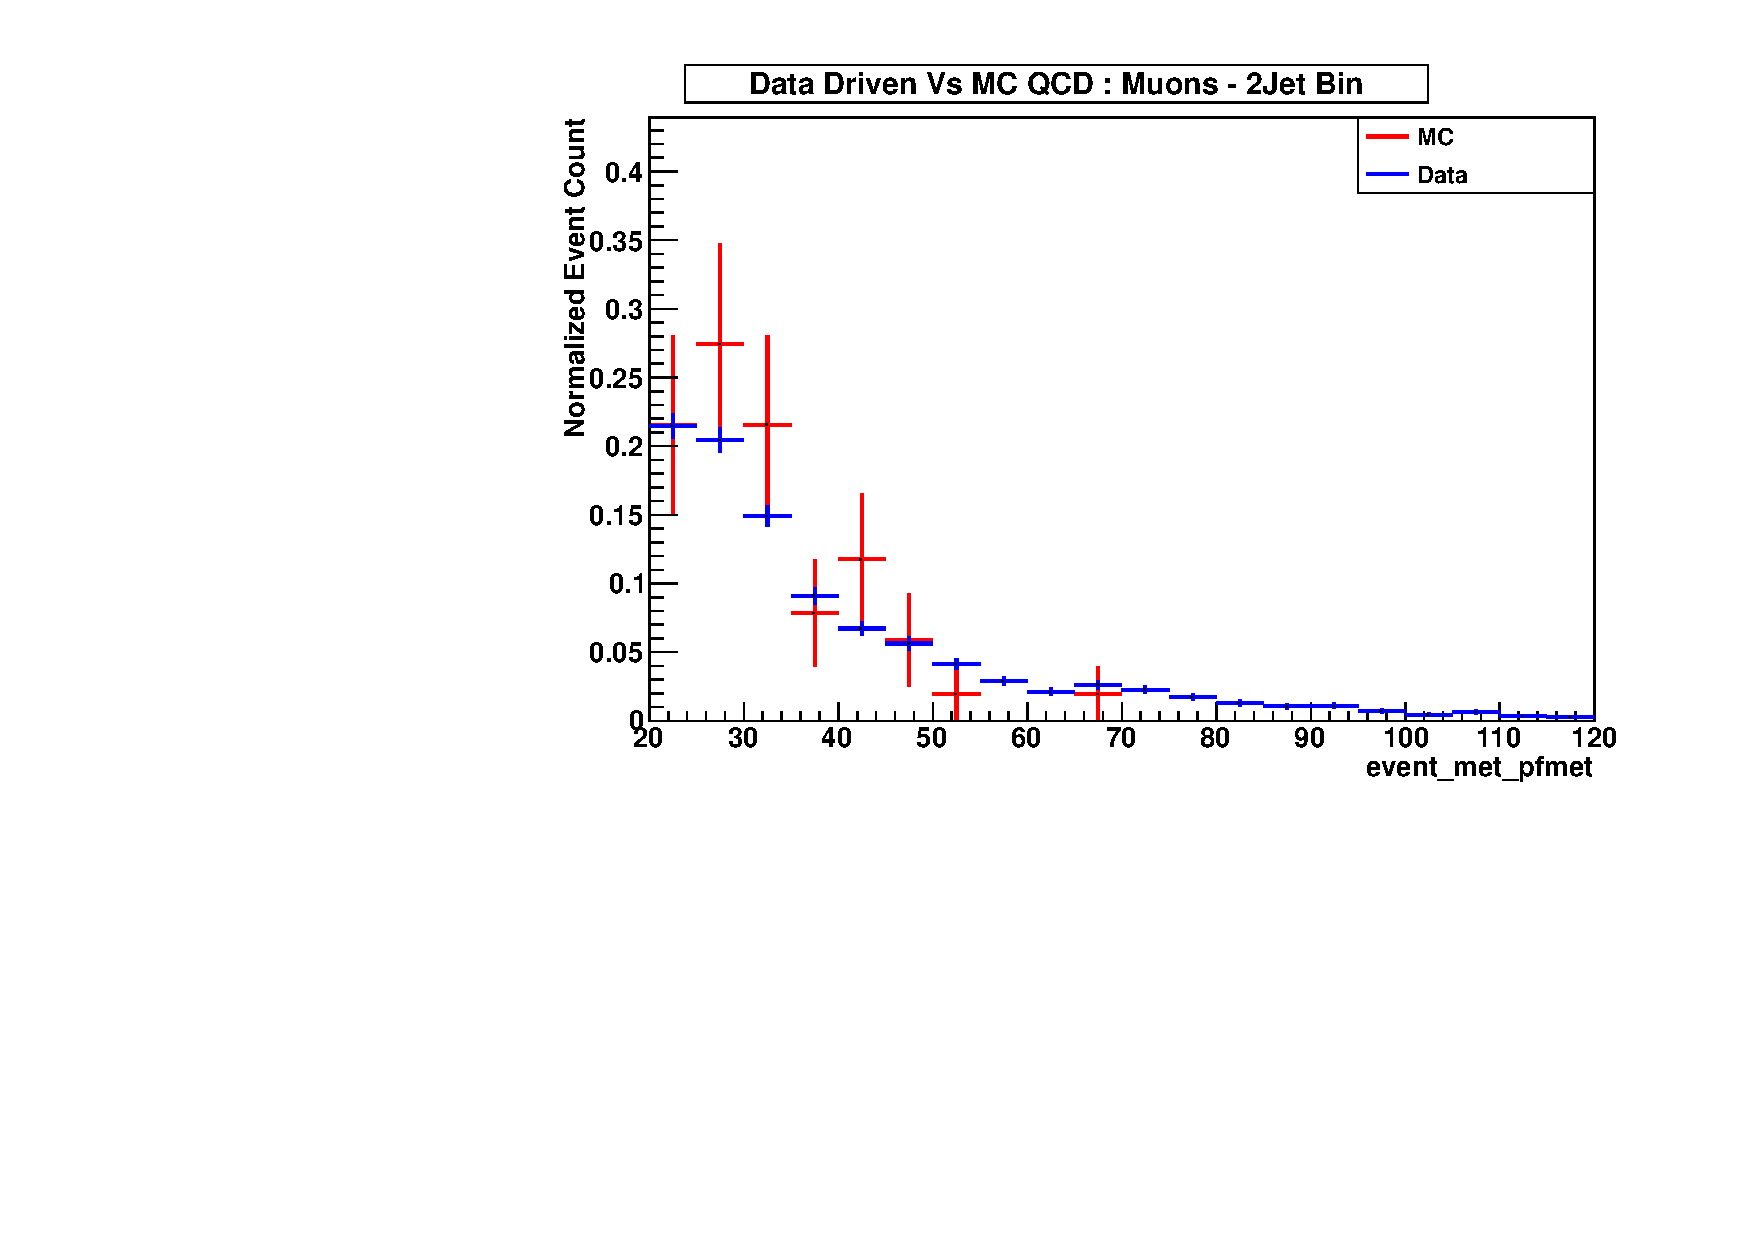
\includegraphics[width=0.48\textwidth]{plots/2012_QCD/QCDDataVSMC_Muons2J_MET.pdf}
%\caption{ Comparison of the MET shapes for MC vs data-driven muon QCD events in the 2-jet bin. The two are statistically consistent.}
%\label{fig:QCDCutLoosening_MET}
%}
%\end{figure}
%%%%%%%
%%%%%%%
\begin{figure}[h!] {\centering
\unitlength=0.33\linewidth
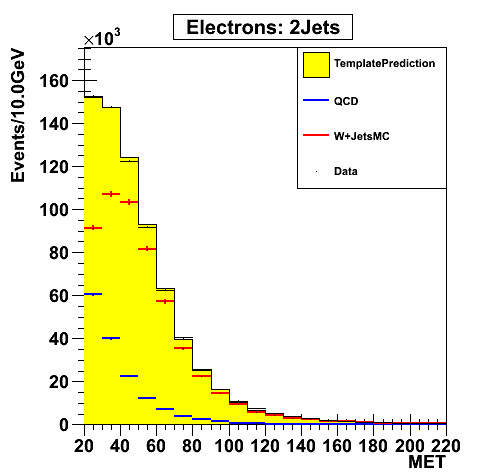
\includegraphics[width=0.90\textwidth]{plots/qcd/TemplateFit9p3fb_MET_el2j.png}
%\put(-0.80,0.0){(a)}
%\unitlength=0.33\linewidth
%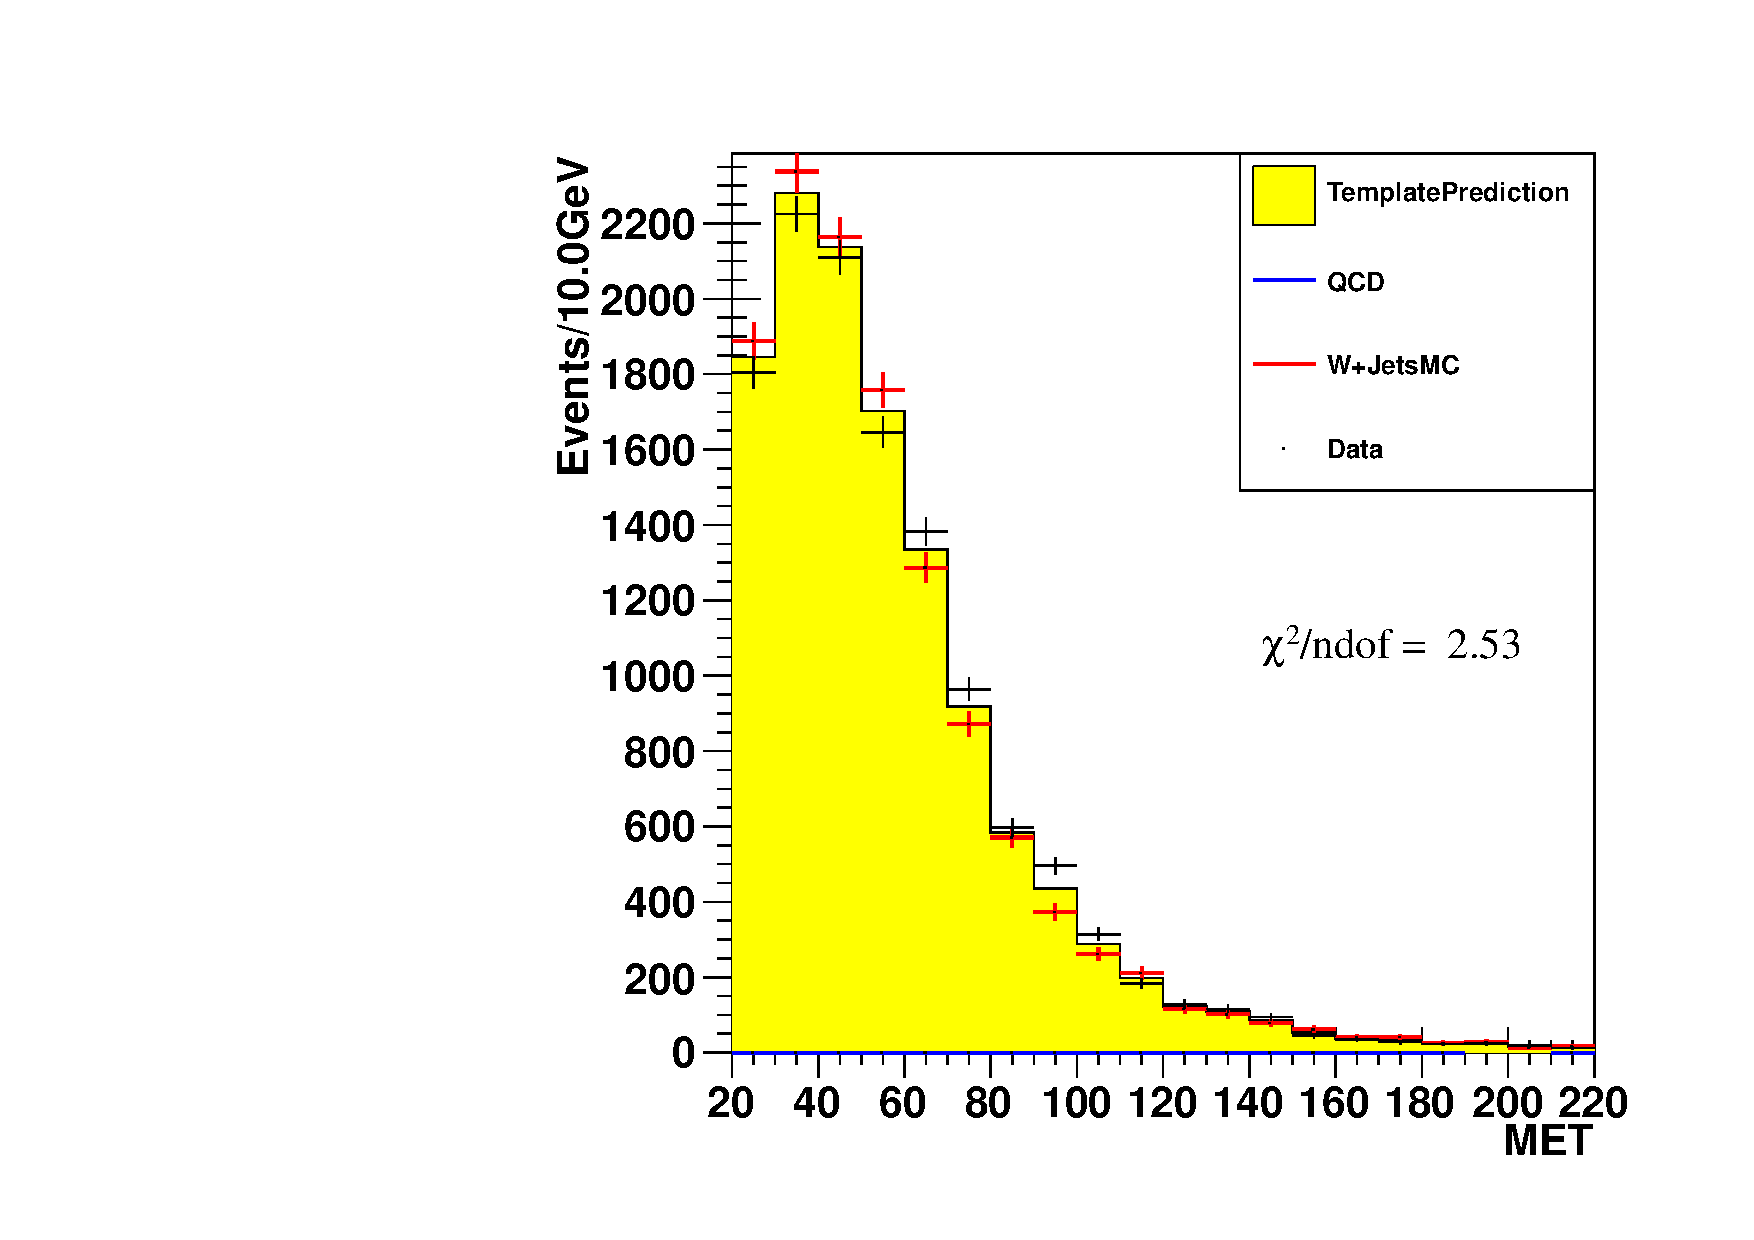
\includegraphics[width=0.48\textwidth]{plots/2012_QCD/TemplateFit_MET_mu3j.pdf}
%\put(-0.80,0.0){(b)} \\
%\unitlength=0.33\linewidth
%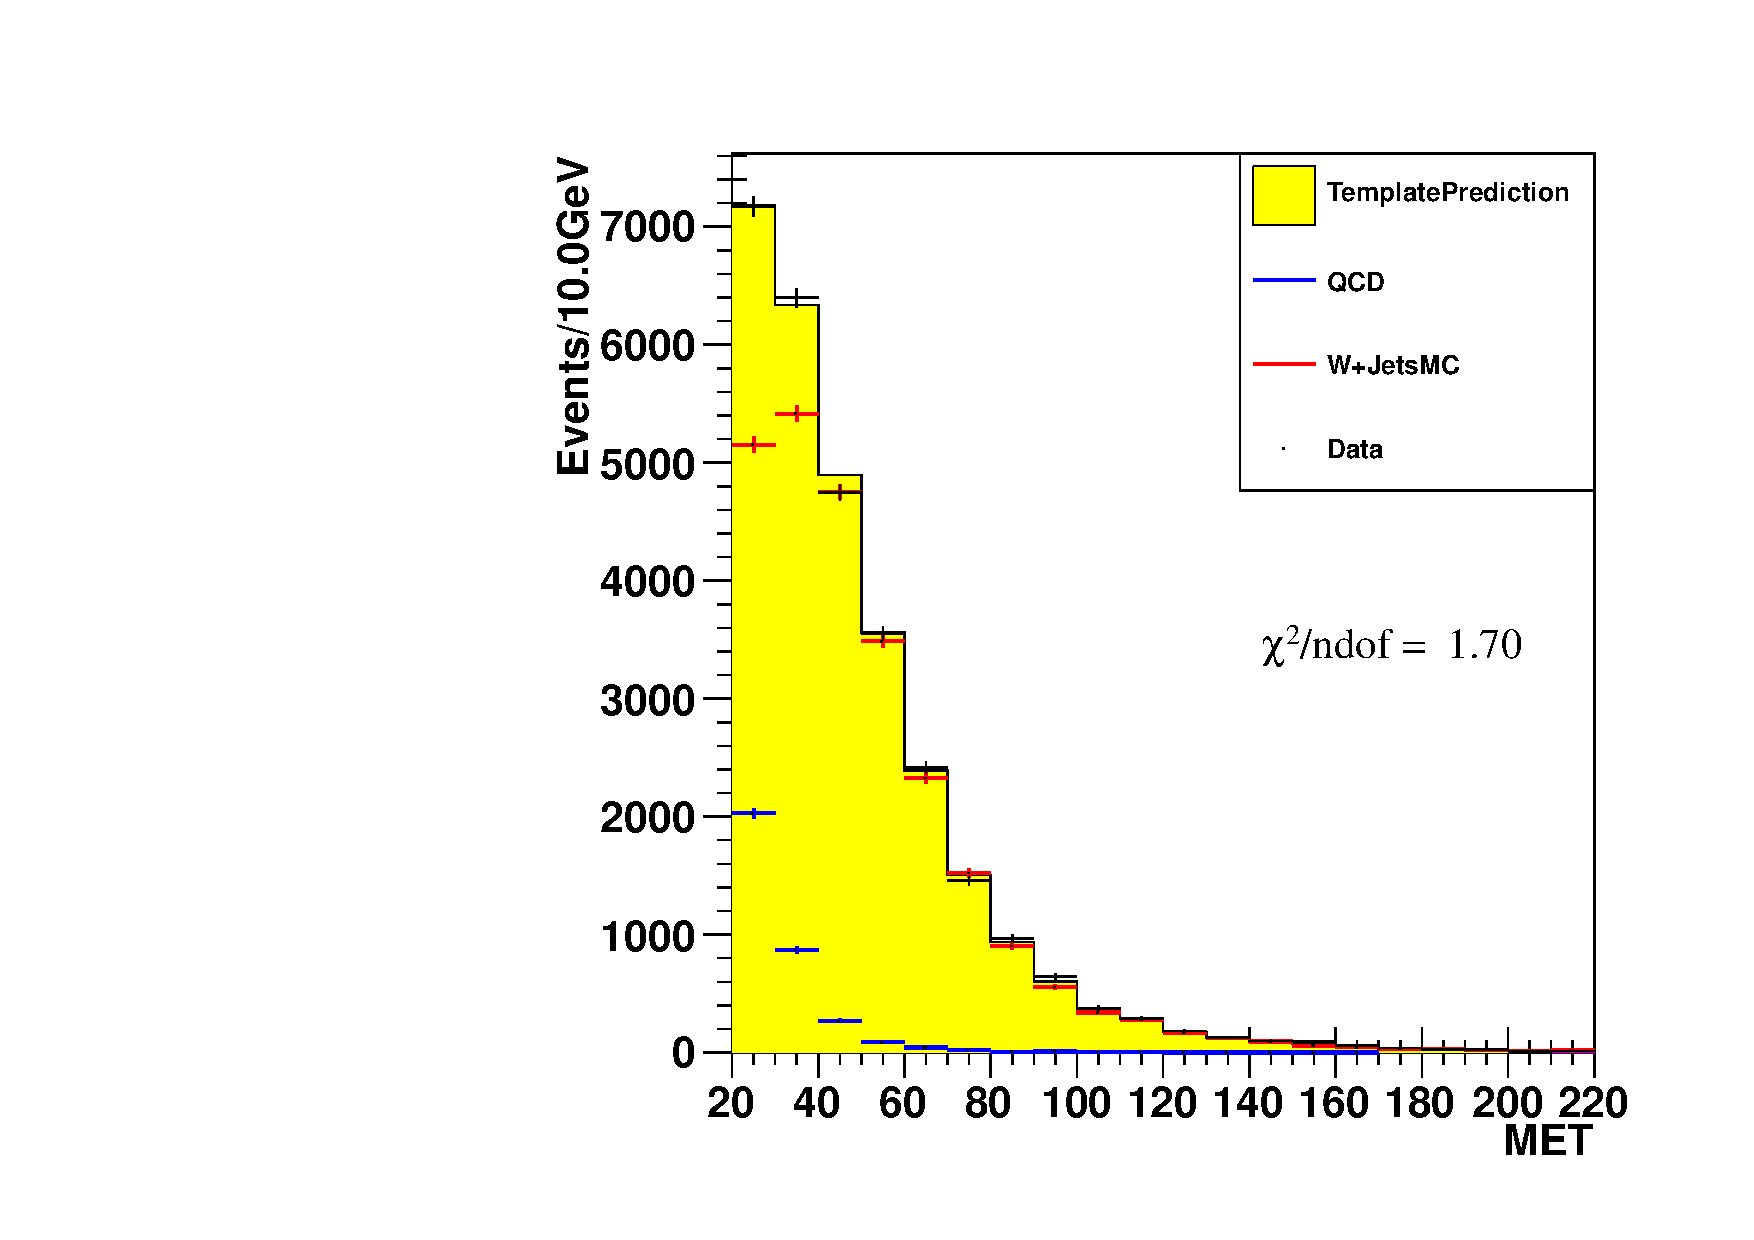
\includegraphics[width=0.48\textwidth]{plots/2012_QCD/TemplateFit_MET_el2j.pdf}
%\put(-0.80,0.0){(c)}
%\unitlength=0.33\linewidth
%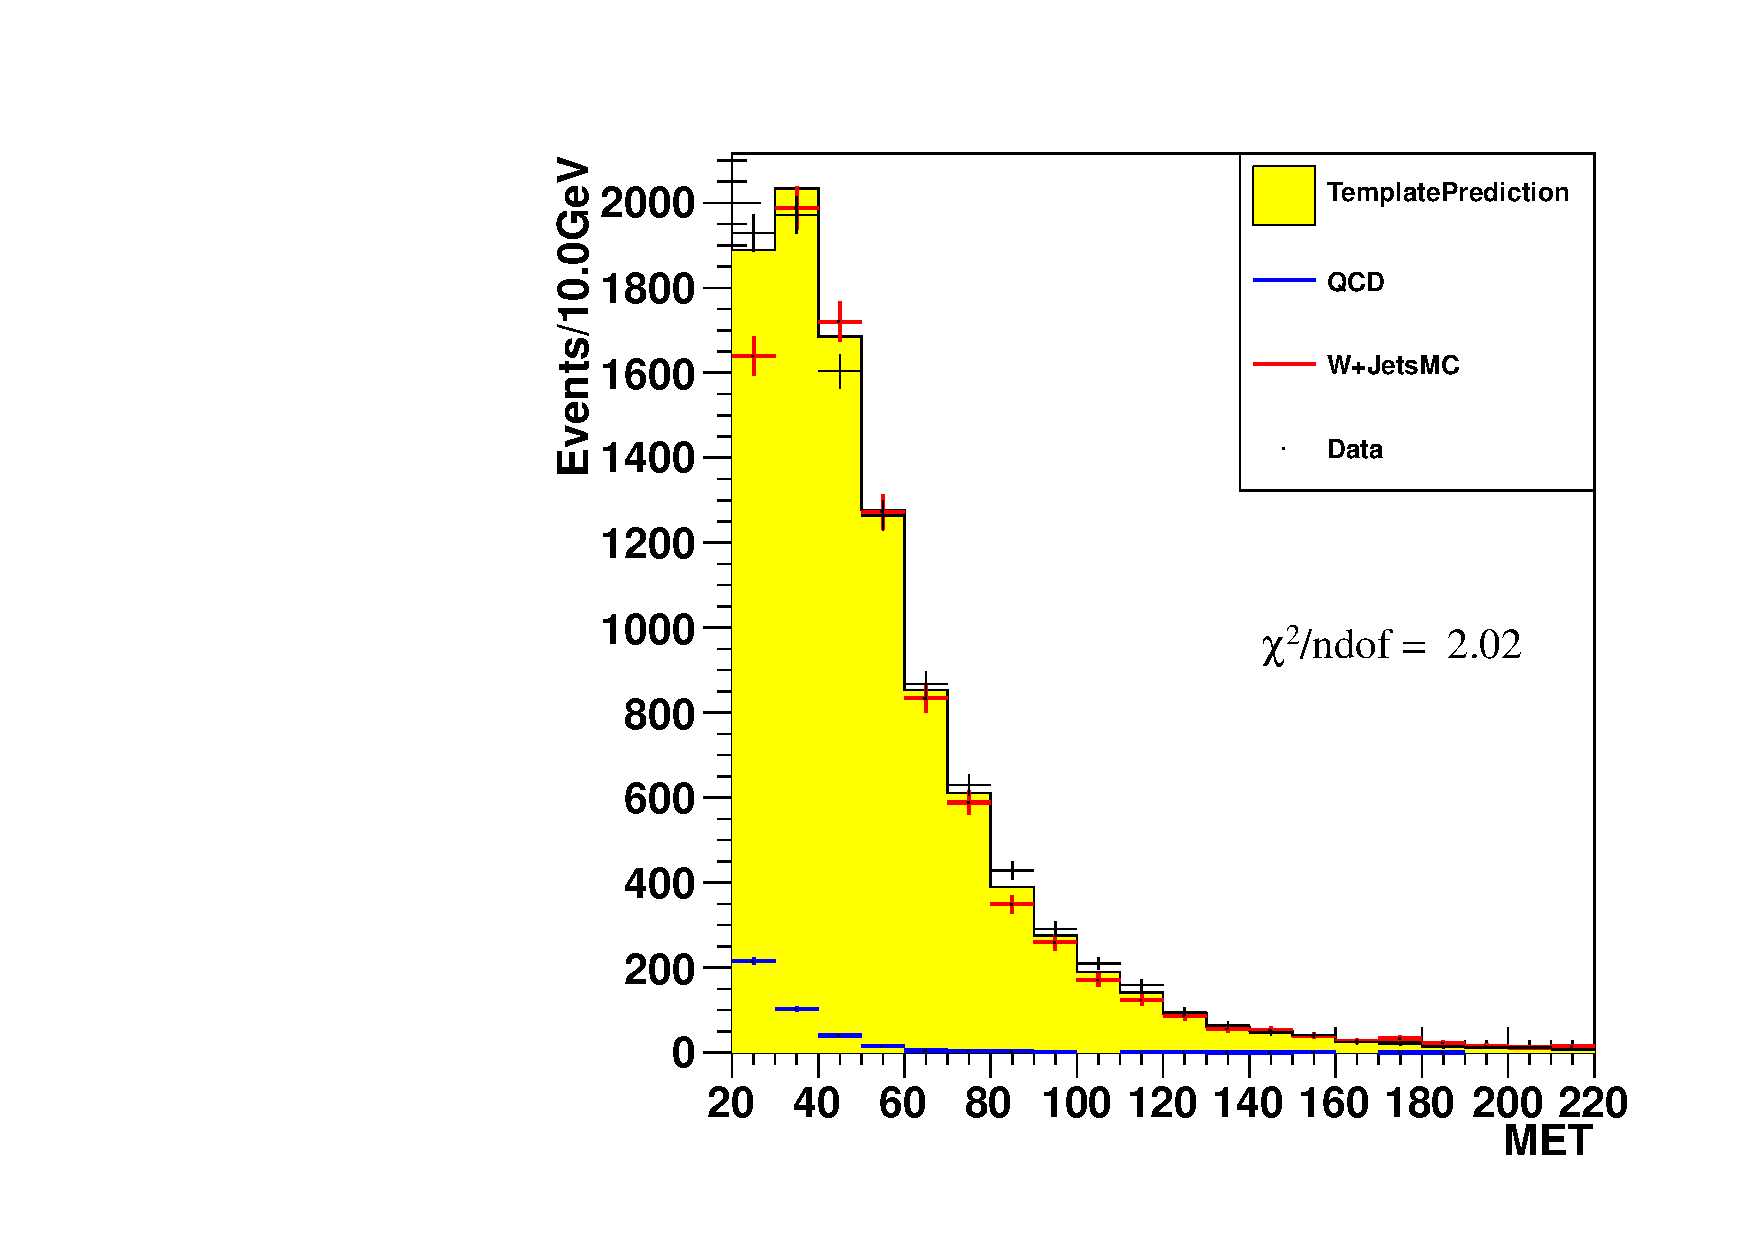
\includegraphics[width=0.48\textwidth]{plots/2012_QCD/TemplateFit_MET_el3j.pdf}
%\put(-0.80,0.0){(d)}
\caption{MET distributions fit to the QCD and W$jj$ templates for electrons.}
\label{fig:QCDTemplateFit_MET}
}
\end{figure}
%%%%%%%
%%%%%%%
\begin{figure}[h!] {\centering
\unitlength=0.33\linewidth
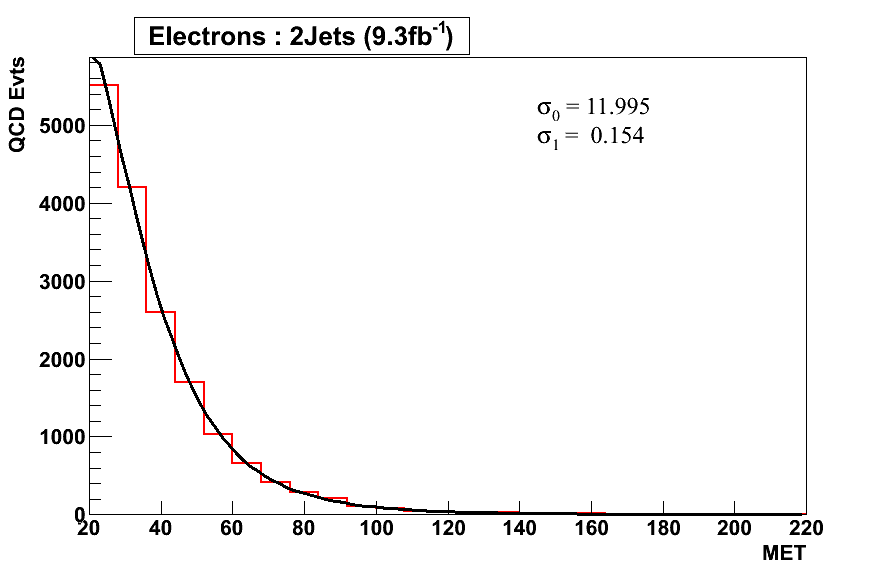
\includegraphics[width=0.90\textwidth]{plots/qcd/RaileighFitQCD_9p3fb_el2j.png}
%\put(-0.80,0.0){(a)}
%\unitlength=0.33\linewidth
%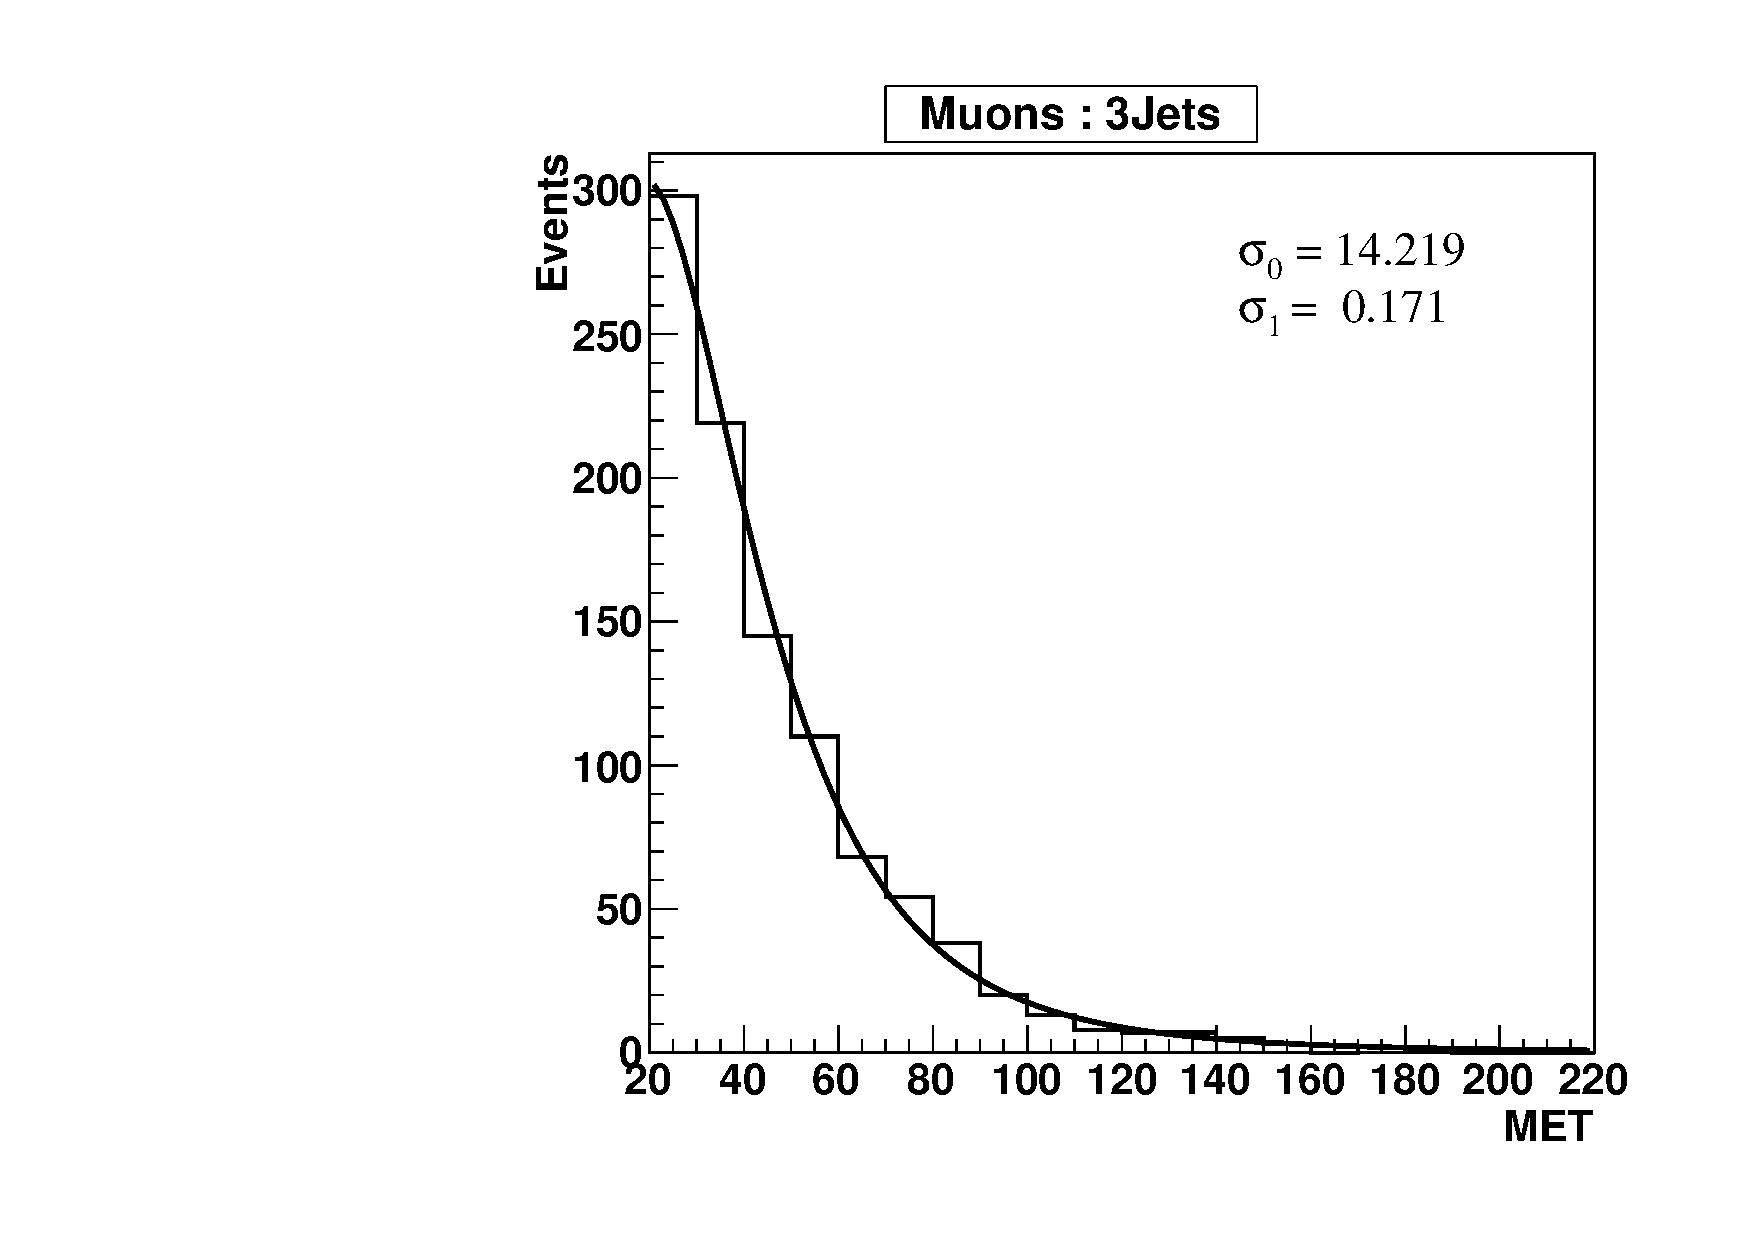
\includegraphics[width=0.48\textwidth]{plots/2012_QCD/RaileighFitQCD_mu3j.pdf}
%\put(-0.80,0.0){(b)} \\
%\unitlength=0.33\linewidth
%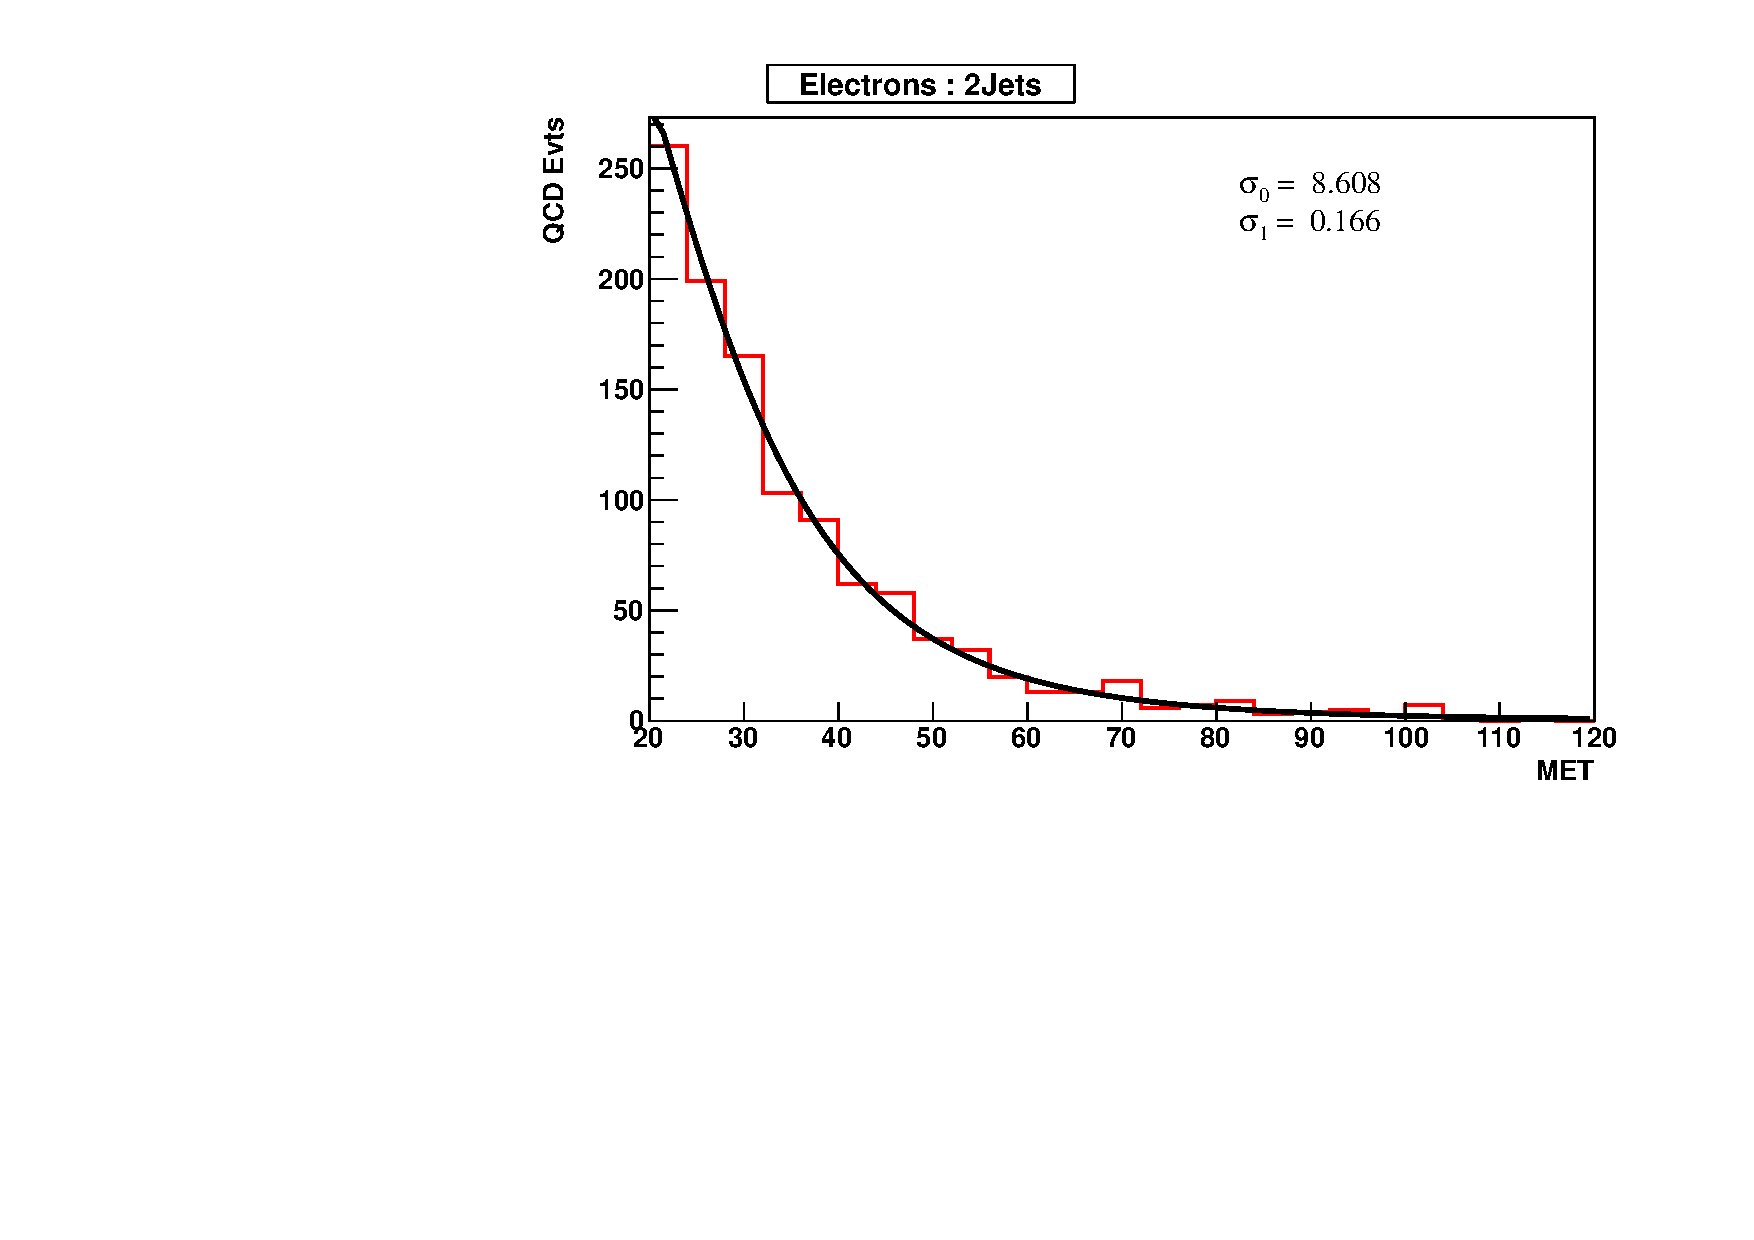
\includegraphics[width=0.48\textwidth]{plots/2012_QCD/RaileighFitQCD_el2j.pdf}
%\put(-0.80,0.0){(c)}
%\unitlength=0.33\linewidth
%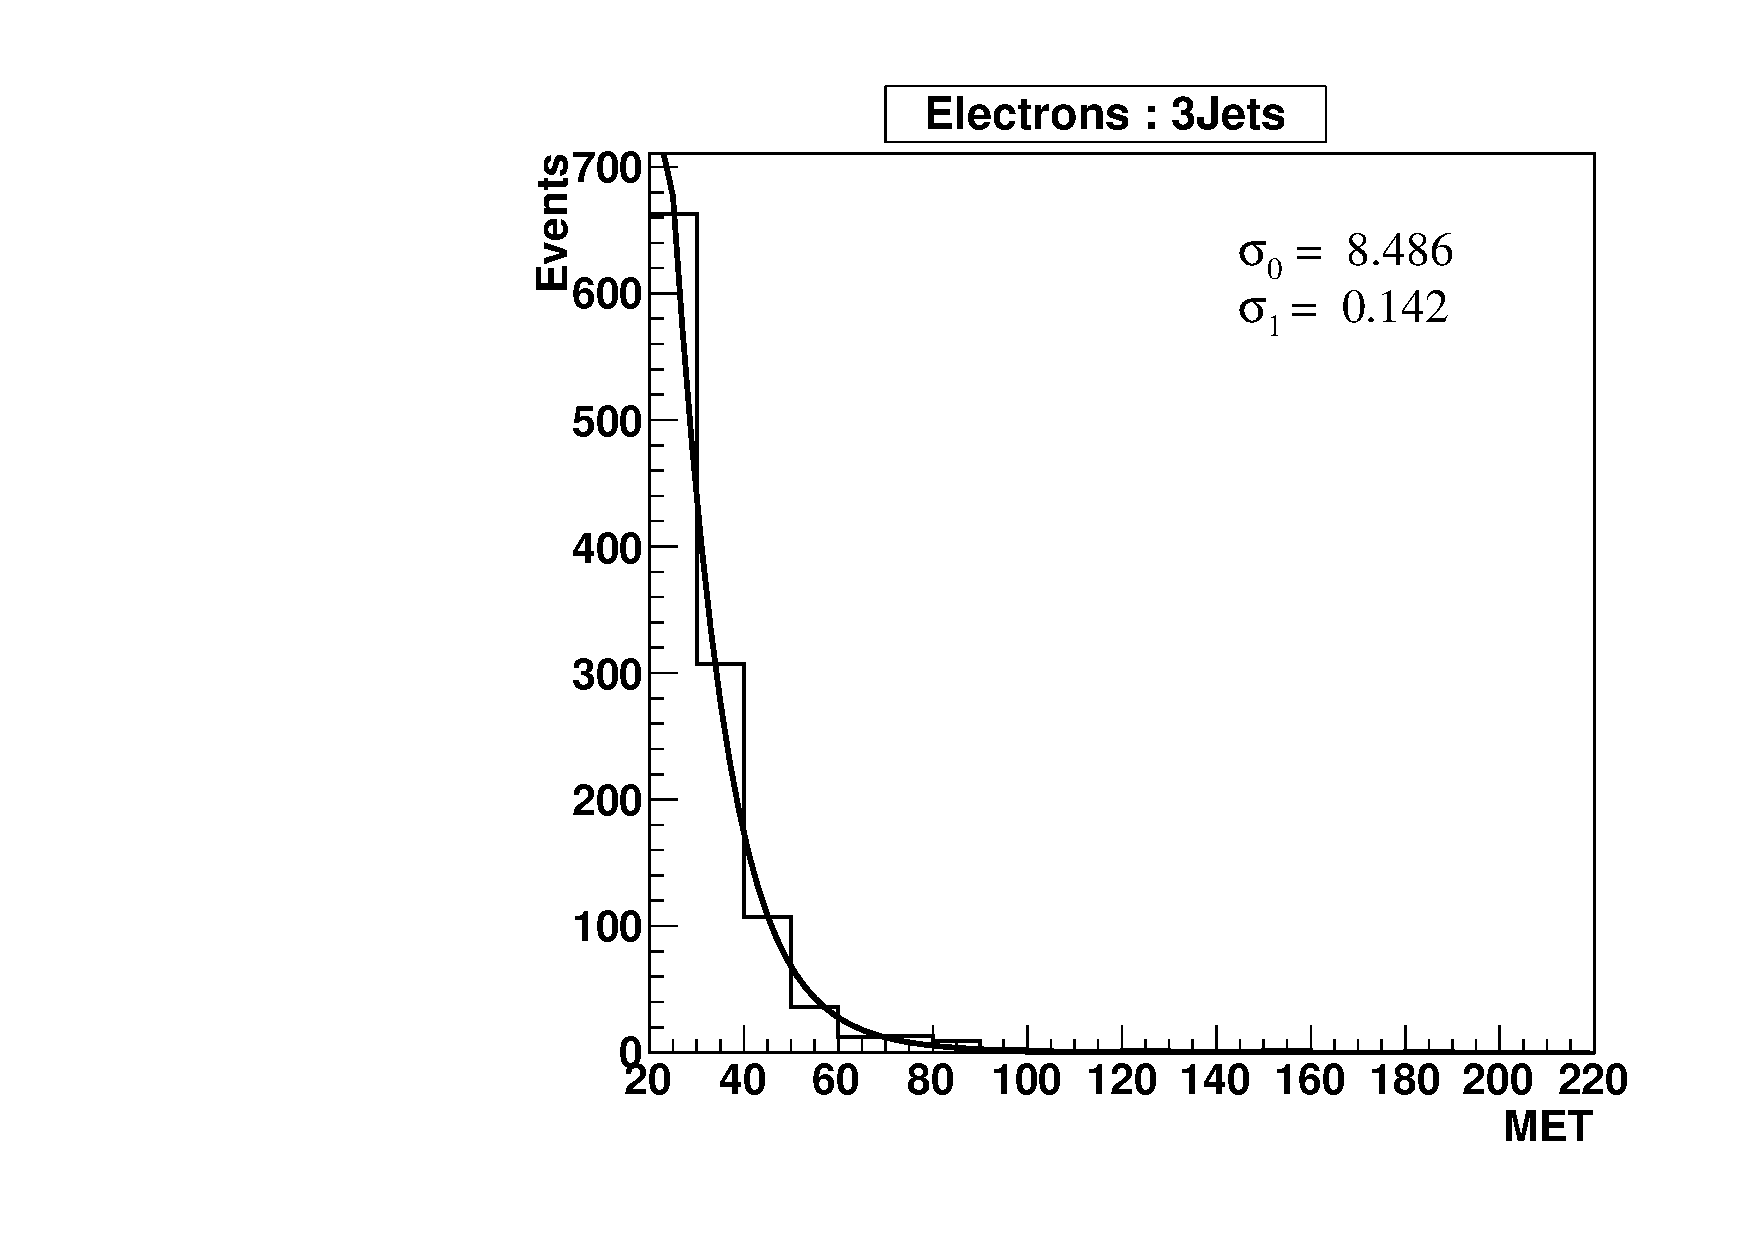
\includegraphics[width=0.48\textwidth]{plots/2012_QCD/RaileighFitQCD_el3j.pdf}
%\put(-0.80,0.0){(d)}
\caption{QCD MET distribution fitted with a Raileigh Function.}
\label{fig:QCDMETRaileighFit}
}
\end{figure}
%%%%%%%
%%%%%%%
% \begin{figure}[h!] {\centering
% \unitlength=0.33\linewidth
% 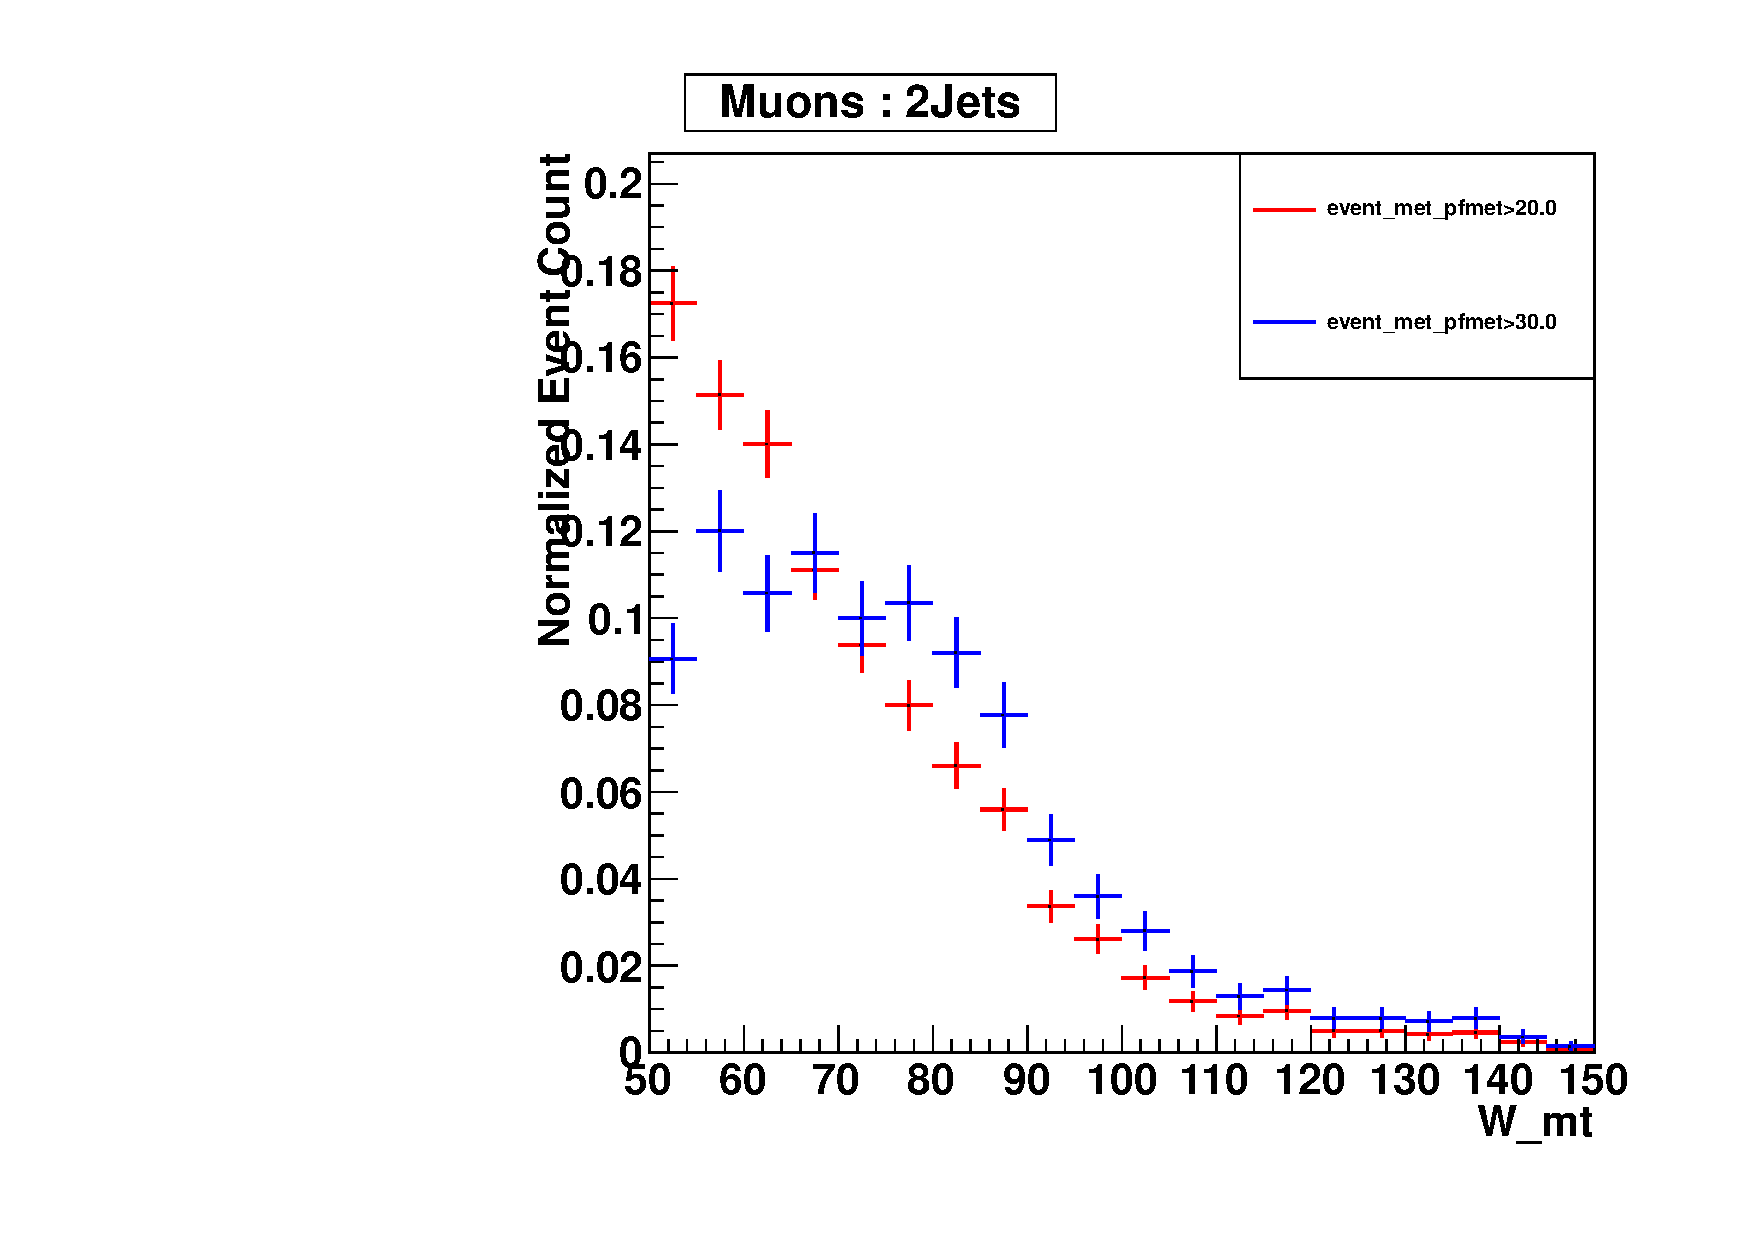
\includegraphics[width=0.48\textwidth]{plots/2012_QCD/METShapeComp_mu2j.pdf}
% \put(-0.80,0.0){(a)}
% \unitlength=0.33\linewidth
% 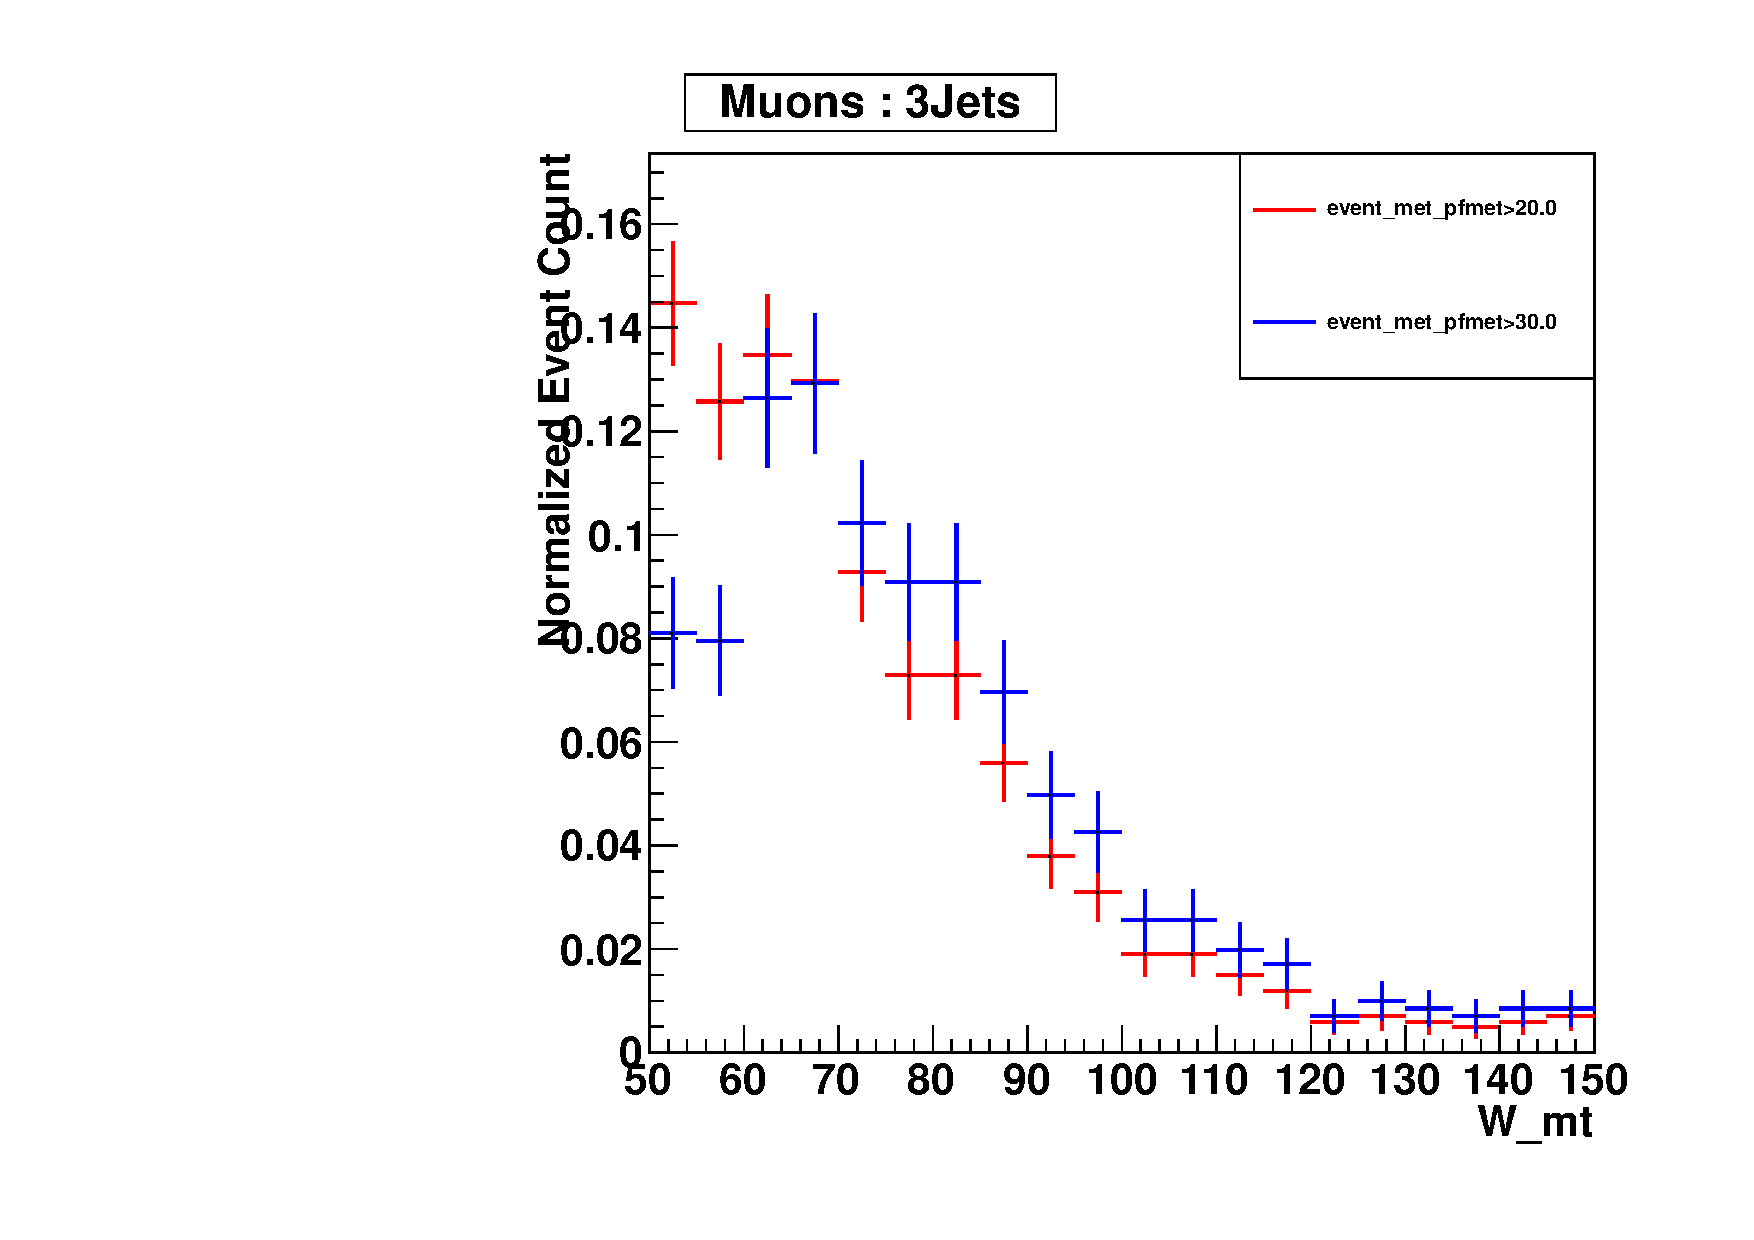
\includegraphics[width=0.48\textwidth]{plots/2012_QCD/METShapeComp_mu3j.pdf}
% \put(-0.80,0.0){(b)} \\
% \unitlength=0.33\linewidth
% 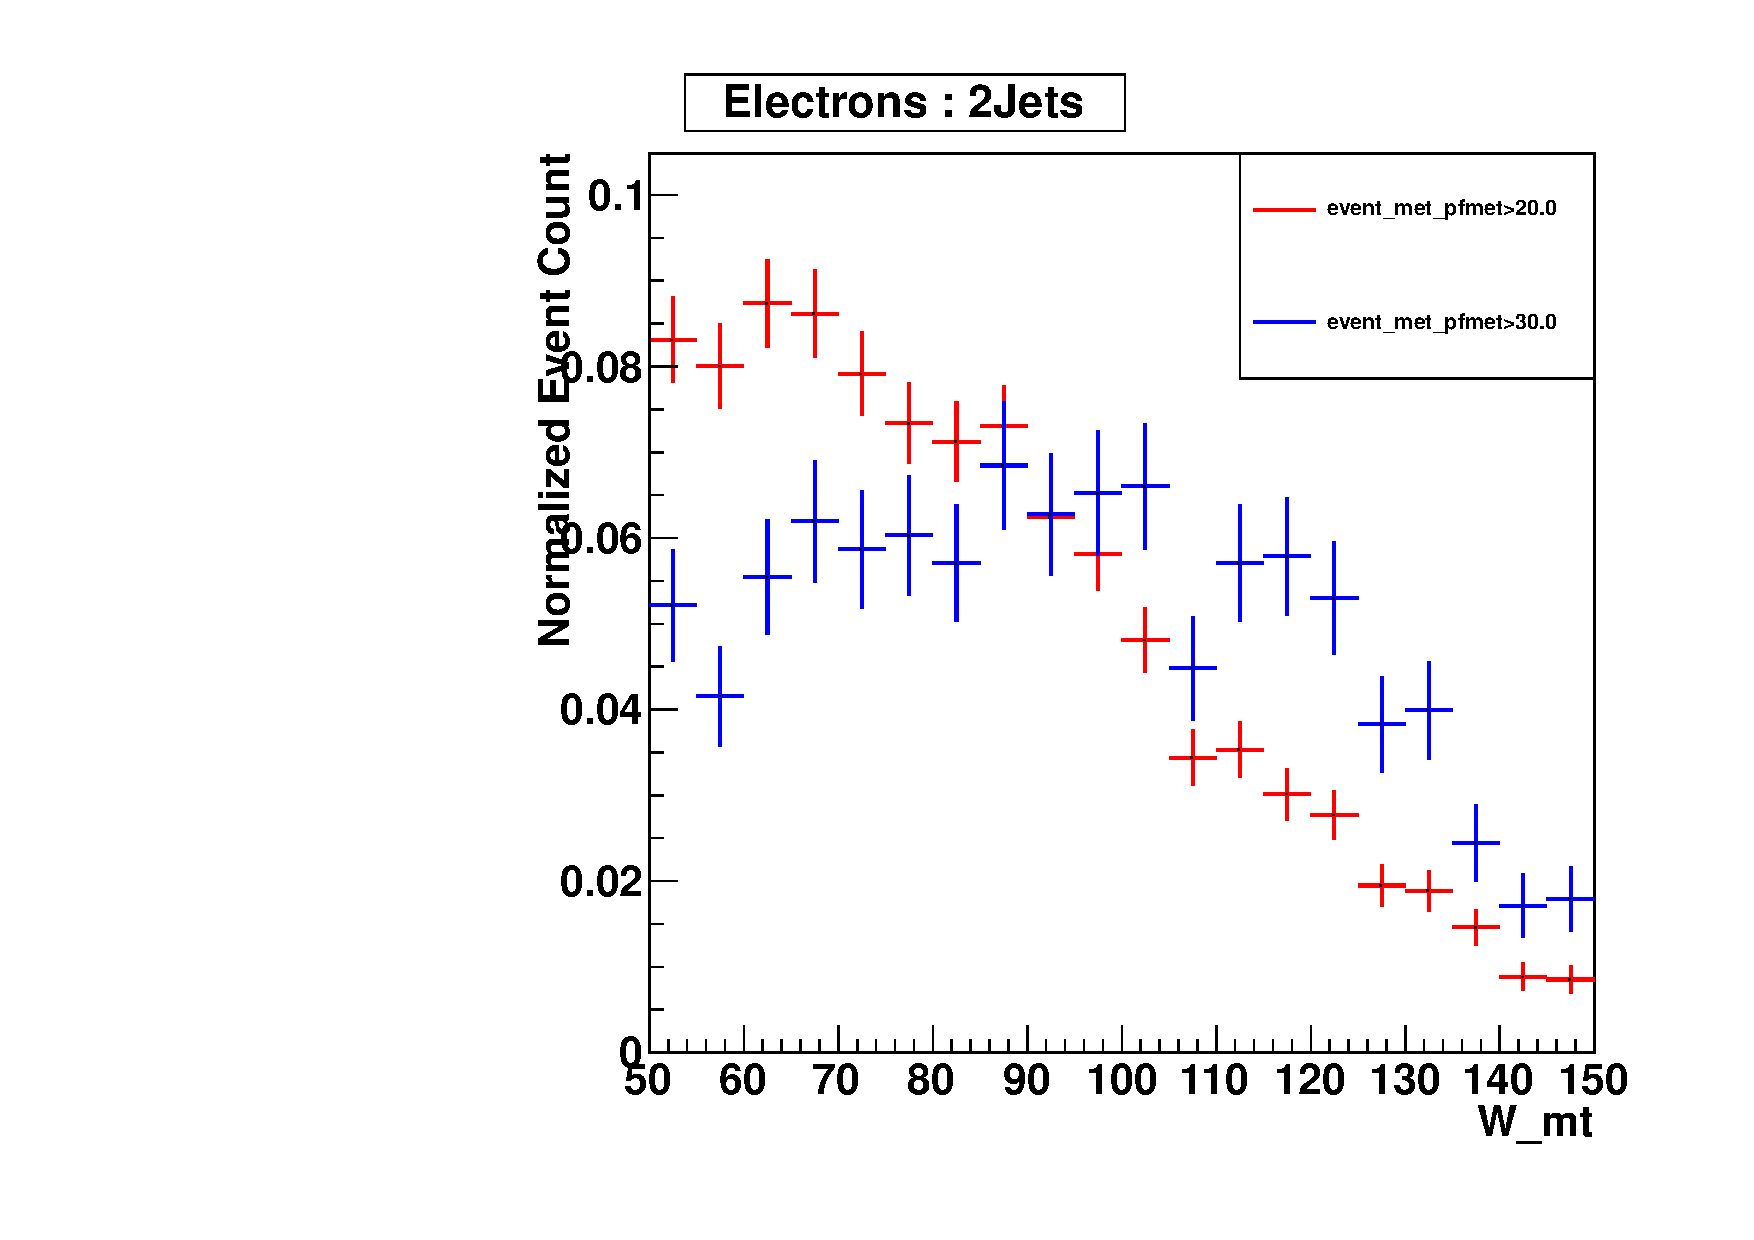
\includegraphics[width=0.48\textwidth]{plots/2012_QCD/METShapeComp_el2j.pdf}
% \put(-0.80,0.0){(c)}
% \unitlength=0.33\linewidth
% 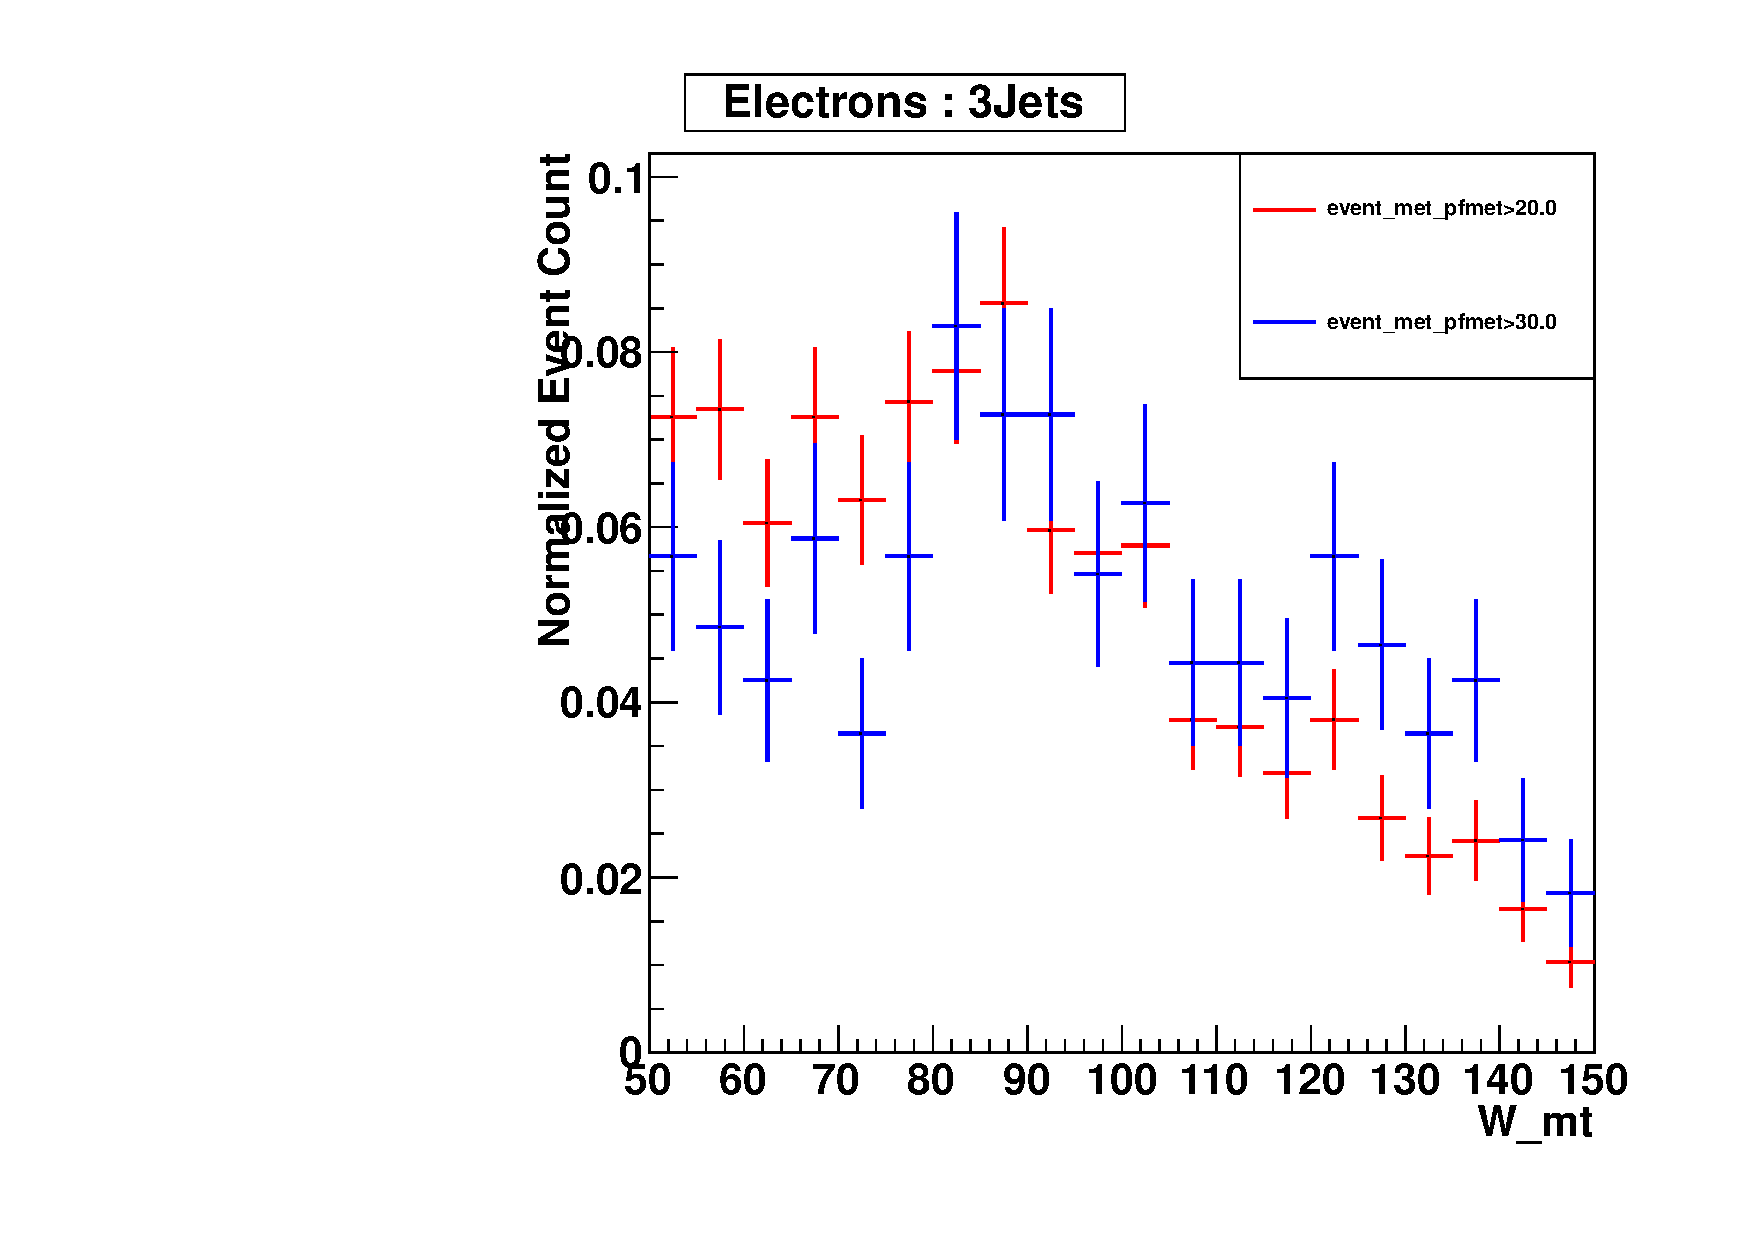
\includegraphics[width=0.48\textwidth]{plots/2012_QCD/METShapeComp_el3j.pdf}
% \put(-0.80,0.0){(d)}
% \caption{ QCD W transverse mass shapes with MET$>20$~GeV vs MET$>30$~GeV for: (a) muons - 2-jet bin, (b) muons - 3-jet bin, (c) electrons - 2-jet bin, (d) electrons - 3-jet bin.}
% \label{fig:QCDMETCutsWmTShape}
% }
% \end{figure}
%%%%%%%
%%%%%%%
\begin{figure}[h!] {\centering
\unitlength=0.33\linewidth
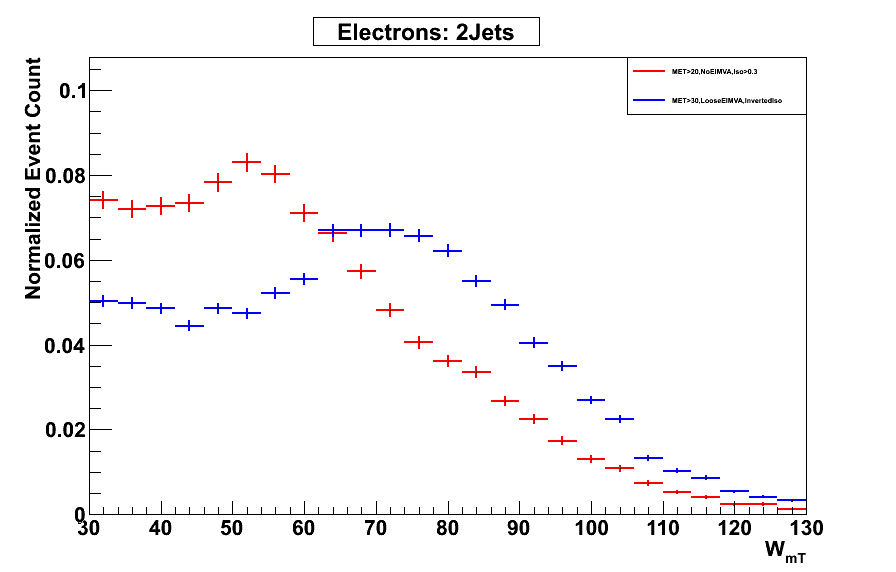
\includegraphics[width=0.90\textwidth]{plots/qcd/El2J_9p3fb_CutComparison_WmT.png}
% \put(-0.80,0.0){(a)}
% \unitlength=0.33\linewidth
% 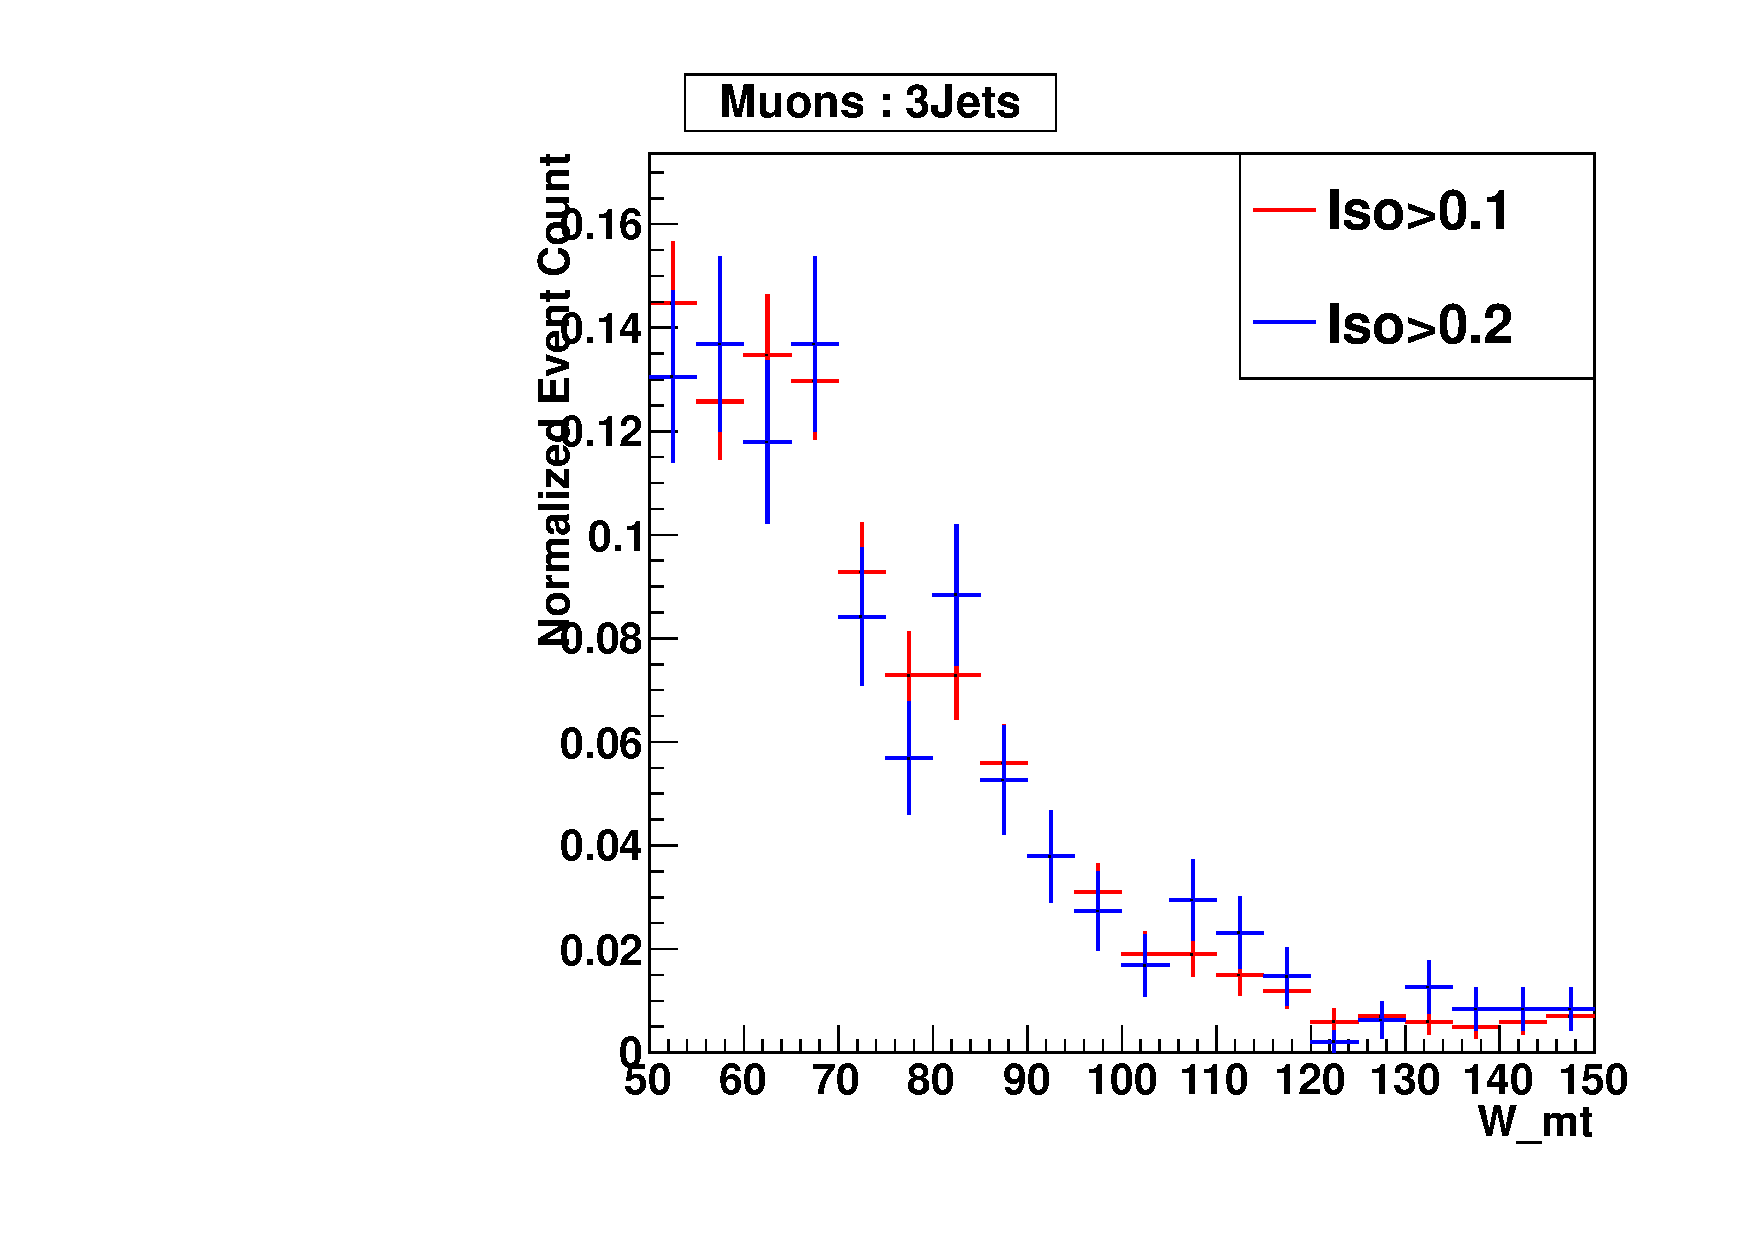
\includegraphics[width=0.48\textwidth]{plots/2012_QCD/ISOShapeComp_WmT_mu3j_g01vg02.pdf}
% \put(-0.80,0.0){(b)} \\
% \unitlength=0.33\linewidth
% 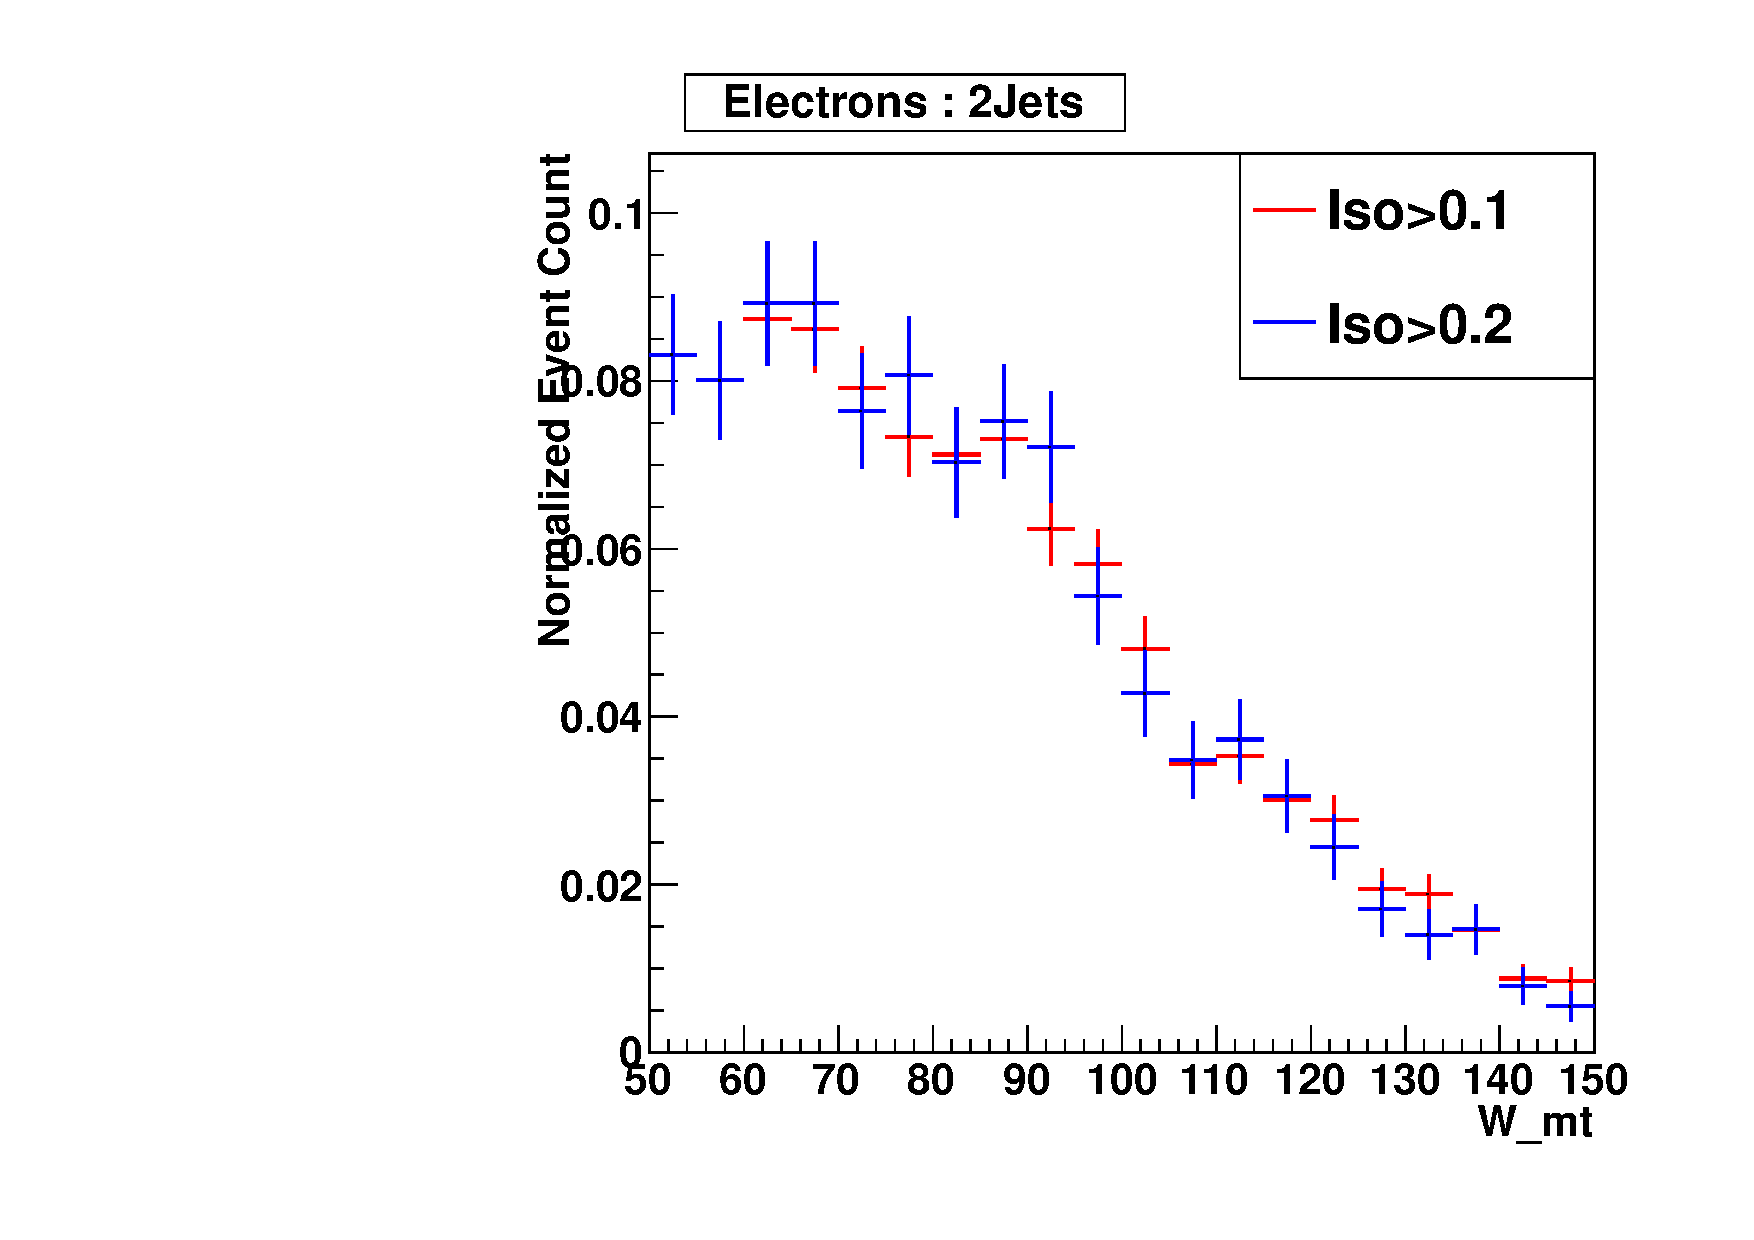
\includegraphics[width=0.48\textwidth]{plots/2012_QCD/ISOShapeComp_WmT_el2j_g01vg02.pdf}
% \put(-0.80,0.0){(c)}
% \unitlength=0.33\linewidth
% 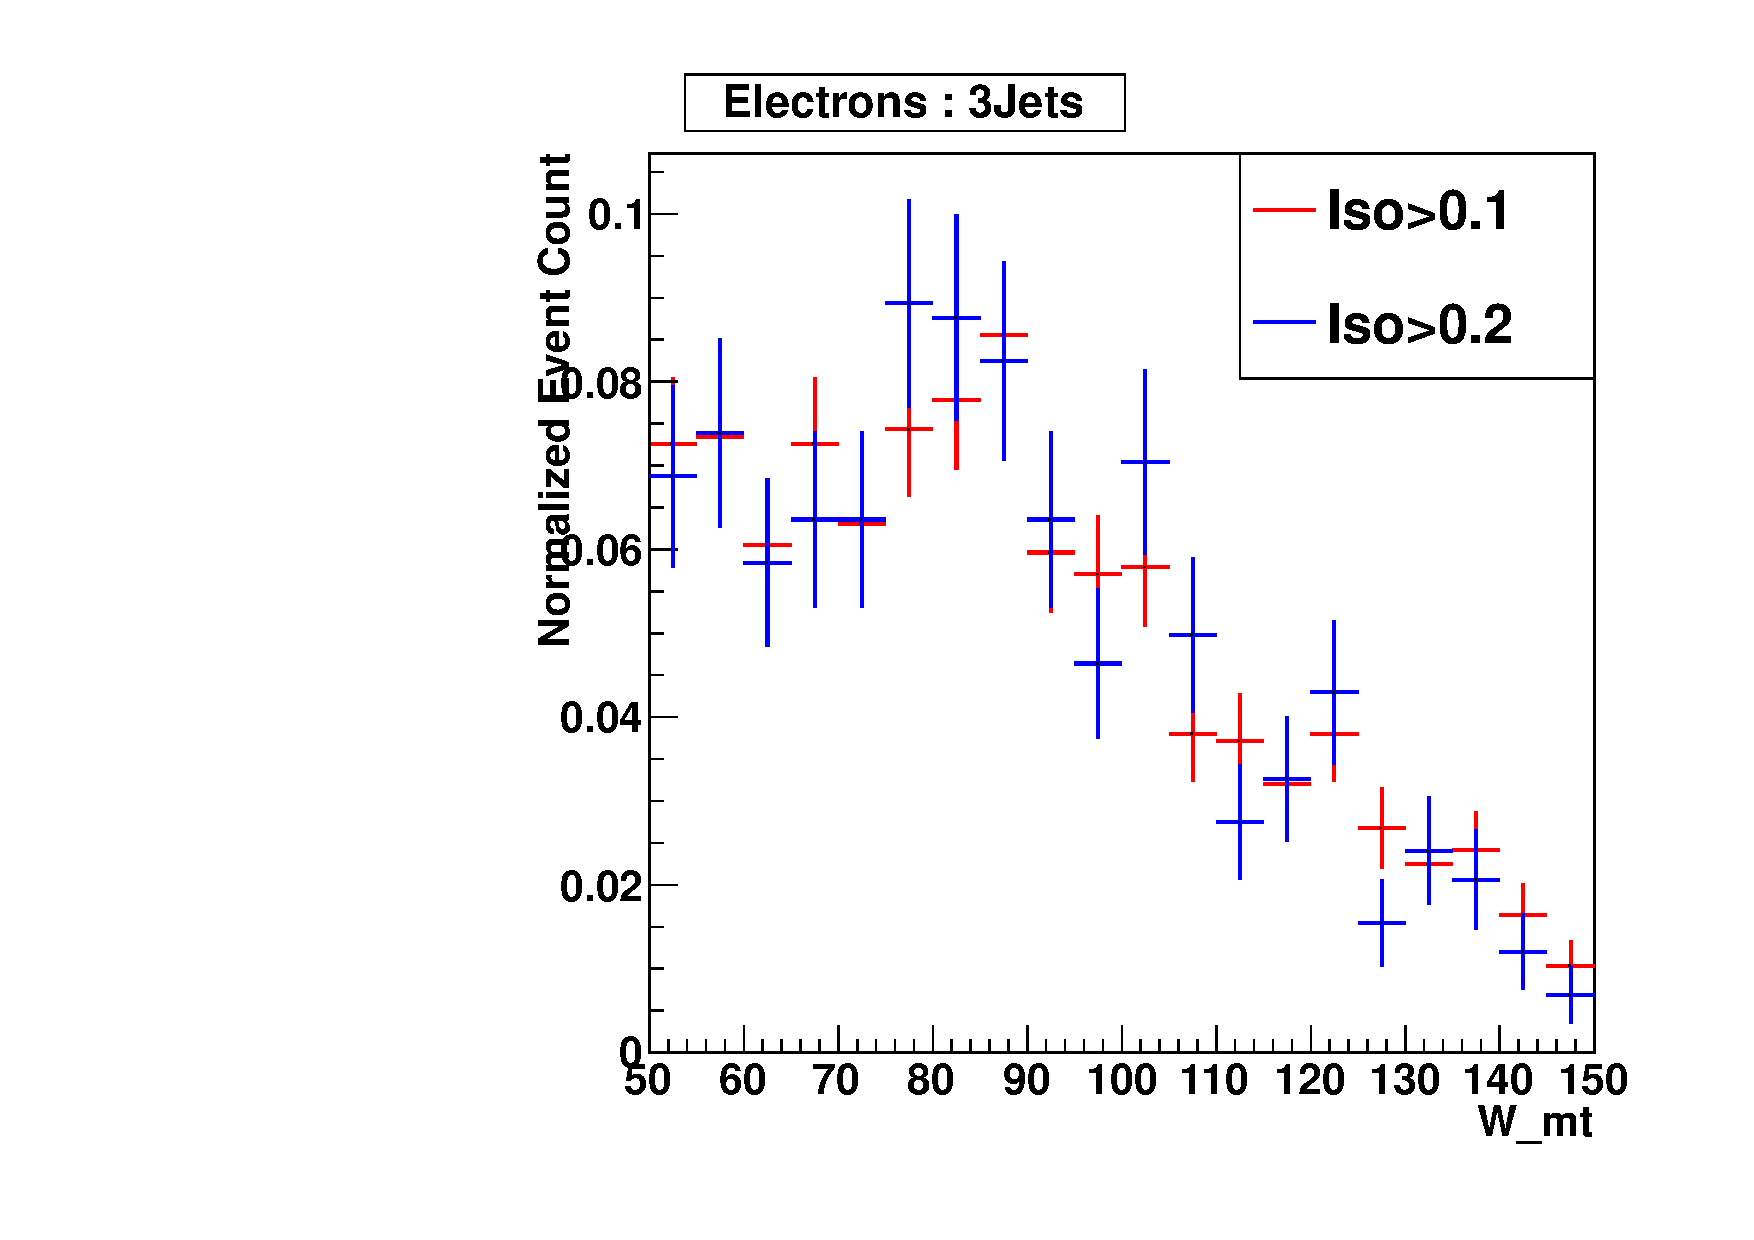
\includegraphics[width=0.48\textwidth]{plots/2012_QCD/ISOShapeComp_WmT_el3j_g01vg02.pdf}
% \put(-0.80,0.0){(d)}
\caption{ QCD W transverse mass shapes with Iso$>0.3$, MET$>20$ and no Electron MVA cut vs inverted loose isolation, MET$>30$ and loose Electron MVA cuts.}
\label{fig:QCDISOCutsWmTShape}
}
\end{figure}
%%%%%%%
%%%%%%%
\begin{figure}[h!] {\centering
\unitlength=0.33\linewidth
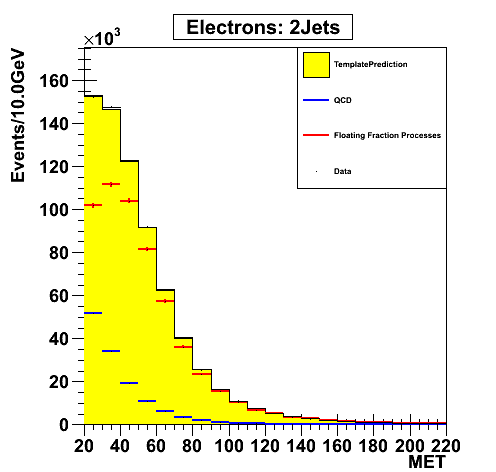
\includegraphics[width=0.48\textwidth]{plots/qcd/TemplateFit9p3fb_MET_AllBkgds_el2j.png}
\put(-0.80,0.0){(a)}
\unitlength=0.33\linewidth
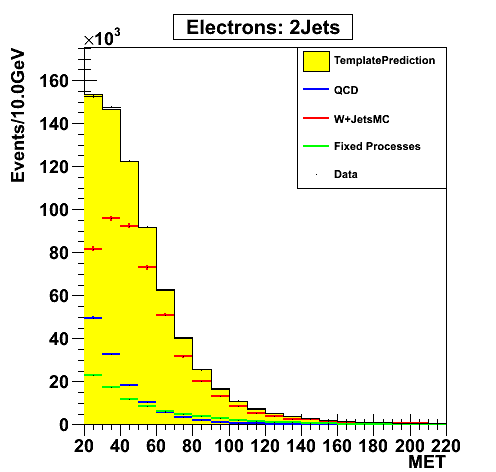
\includegraphics[width=0.48\textwidth]{plots/qcd/TemplateFit9p3fb_MET_AllBkgdsFixNonWpJ_el2j.png}
\put(-0.80,0.0){(b)}
\caption{ Electron MET distribution fit with: (a) fractions of the non QCD processes fixed relative to each other and the overall coefficient allowed to float (b) the additional backgrounds (i.e. processes which are not W+Jets or QCD) fixed to their expected yields and W+Jets (as well as QCD) fraction allowed to float. The resultant fraction of QCD events is consistent with the default approach (Fig.~\ref{fig:QCDTemplateFit_MET}).}
\label{fig:QCDTemplateFit_MET_AllBkgds}
}
\end{figure}
%%%%%%%